\documentclass{beamer}
\usetheme[numbering=none]{metropolis}
\def\notescolors{1}
% specifications for presenter mode
%\beamerdefaultoverlayspecification{<+->}
%\setbeamercovered{transparent}

\usepackage[english]{babel}
\usepackage[utf8x]{inputenc}

%\usepackage{coloremoji}
\usepackage{layout}
\usepackage{multirow}
\usepackage{array}
\usepackage{graphicx}
\graphicspath{ {figs/} }

\setbeameroption{hide notes}
\setbeamertemplate{note page}[plain]
\usepackage{listings}
\usepackage{datetime}
\usepackage{url}
\usepackage{tcolorbox}
\usepackage{appendixnumberbeamer}
\usepackage[normalem]{ulem}

\usepackage{tikz}
\def\checkmark{\tikz\fill[scale=0.4](0,.35) -- (.25,0) -- (1,.7) -- (.25,.15) -- cycle;}

% math shorthand
\usepackage{bm}
\usepackage{amsthm}
\usepackage{amstext}
\usepackage[font=small]{caption}
\usepackage{amsmath}
\usepackage{mathtools}
\usepackage{cancel}
\DeclareMathOperator{\logit}{logit}
\newcommand{\R}{\mathbb{R}}
\newcommand{\D}{\mathcal{D}}
\newcommand{\E}{\mathbb{E}}
\newcommand{\I}{\mathbb{I}}
\newcommand{\pr}{\mathbb{P}}
\newcommand{\F}{\mathcal{F}}
\newcommand{\X}{\mathcal{X}}
\newcommand{\M}{\mathcal{M}}
\newcommand{\lik}{\mathcal{L}}

\newtheorem*{assumption*}{\assumptionnumber}
\providecommand{\assumptionnumber}{}
\makeatletter
\newenvironment{assumption}[2]
 {%
  \renewcommand{\assumptionnumber}{Assumption #1: $\mathcal{#2}$}%
  \begin{assumption*}%
  \protected@edef\@currentlabel{#1: $\mathcal{#2}$}%
 }
 {%
  \end{assumption*}
 }
\makeatother

\DeclarePairedDelimiterX{\infdivx}[2]{(}{)}{%
  #1\;\delimsize\|\;#2%
}
\newcommand{\infdiv}{D\infdivx}
\DeclarePairedDelimiter{\norm}{\lVert}{\rVert}
\DeclareMathOperator*{\argmin}{arg\,min}
\DeclareMathOperator*{\argmax}{arg\,max}

% indepndence notation macro
\newcommand\indep{\protect\mathpalette{\protect\independenT}{\perp}}
\def\independenT#1#2{\mathrel{\rlap{$#1#2$}\mkern2mu{#1#2}}}

% Bibliography
\usepackage{natbib}
\bibpunct{(}{)}{,}{a}{}{;}
%\usepackage{bibentry}

% highlight name in bibliography
\usepackage{xstring}
\def\FormatName#1{%
  \IfSubStr{#1}{Hejazi}{\underline{\textbf{#1}}}{#1}%
}


\title{\normalsize Causal machine learning to analyze vaccine efficacy
  trials: Biostatistics on the frontiers of a public health nightmare}
\author{\href{https://nimahejazi.org}{Nima Hejazi}\\[-10pt]}
\institute{
  \begin{figure}[!htb]
    \centering
    \begin{minipage}{0.65\textwidth}
        Department of Biostatistics,\\
        T.H.~Chan School of Public Health,\\
        Harvard University\\[6pt]
        
\includegraphics[scale=0.12]{twitter-icon.png}
          \href{https://twitter.com/nshejazi}{nshejazi} \\
        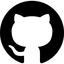
\includegraphics[scale=0.09]{github-icon.png}
          \href{https://github.com/nhejazi}{nhejazi} \\
        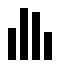
\includegraphics[scale=0.12]{homepage.png}
          \href{https://nimahejazi.org}{nimahejazi.org} \\
     Biostatistics Lightning Talk,\\Harvard T.H.~Chan School of Public Health
    \end{minipage}%
    \begin{minipage}{0.3\textwidth}
      \centering
      \vspace{-60pt}
      
\includegraphics[width=1.1in]{hsph}
    \end{minipage}
  \end{figure}
}

\date{Thursday, 06 October 2022}

%%%%%%%%%%%%%%%%%%%%%%%%%%%%%%%%%%%%%%%%%%%%%%%%%%%%%%%%%%%%%%%%%%%%%%%%%%%%%%%%

% Outline at beginning of each section
%\AtBeginSection[]
%{
  %\begin{frame}<beamer>
    %\frametitle{Outline}
    %\tableofcontents[currentsection]
  %\end{frame}
%}

%%%%%%%%%%%%%%%%%%%%%%%%%%%%%%%%%%%%%%%%%%%%%%%%%%%%%%%%%%%%%%%%%%%%%%%%%%%%%%%

\begin{document}

\begin{frame}[noframenumbering]
  \thispagestyle{empty}
  \titlepage

\note{
}

\end{frame}

%%%%%%%%%%%%%%%%%%%%%%%%%%%%%%%%%%%%%%%%%%%%%%%%%%%%%%%%%%%%%%%%%%%%%%%%%%%%%%%%

%\begin{frame}[standout]
  %Immune Correlates of HIV-1 and COVID-19
%\end{frame}

%%%%%%%%%%%%%%%%%%%%%%%%%%%%%%%%%%%%%%%%%%%%%%%%%%%%%%%%%%%%%%%%%%%%%%%%%%%%%%%%

\begin{frame}[c]{The Ongoing Fights Against HIV-1 and COVID-19}

\begin{center}
\begin{itemize}
  \itemsep8pt
  \item The HIV-1 epidemic:
    \begin{itemize}
      \itemsep4pt
      \item 1.5 million new infections occurring annually worldwide;
      \item new infections outpace patients starting antiretroviral therapy;
      %\item $<$40\% efficacy rate for \textit{most efficacious} preventive
        %vaccine.
      \item HIV Vaccine Trials Network's (HVTN) \textit{505} trial evaluated a
        novel antibody boost vaccine~\citep{hammer2013efficacy}.
    \end{itemize}
  \item The COVID-19 \sout{epi}~\sout{pan}~endemic~\citep{antia2021transition}:
    \begin{itemize}
      \itemsep4pt
      \item \sout{270} \sout{331} 619 million total cases have been detected
        globally;
      \item new variants emerging, with vaccine uptake globally slowing;
      %\item $\sim$95\% efficacy rate for \textit{most efficacious} vaccine(s).
      \item COVID-19 Prevention Network's (CoVPN) \textit{COVE} trial focused
        on Moderna's (mRNA-1273) vaccine~\citep{baden2021efficacy}.
    \end{itemize}
  \item \textbf{Question}: How can [HIV-1, COVID-19] vaccines be improved
    through modulating immunogenic response profiles?
\end{itemize}
\end{center}

\note{
\begin{itemize}
  \item Baseline covariates($L$): sex, age, BMI, behavioral HIV risk.
  \item Intervention(s) ($A$): post-vaccination T-cell activity markers.
  \item Outcome ($Y$): HIV-1 infection status at week 28 of tiral.
  \item 12-color intracellular cytokine staining (ICS) assay.
  \item Cryopreserved peripheral blood mononuclear cells were stimulated with
    synthetic HIV-1 peptide pools.
  \item A vaccine effective at preventing HIV-1 acquisition would be a
    cost-effective and durable approach to halting the worldwide epidemic.
  \item The study was halted on 22 April 2013 due to absence of vaccine
    efficacy. There was no significant effect of the vaccine on the primary
    infection endpoint of HIV-1 infection between week 28 and month 24.
\end{itemize}

\begin{itemize}
  \item Did we have the time? Polio (7 years), Measles (9 years),
    Chickenpox (34 years), Mumps (4 years), HPV (15 years).
  \item How did we make it? Typical process timeline (73 months) replaced by an
    \textit{accelerated} process of 14 months.
\end{itemize}
}

\end{frame}

%%%%%%%%%%%%%%%%%%%%%%%%%%%%%%%%%%%%%%%%%%%%%%%%%%%%%%%%%%%%%%%%%%%%%%%%%%%%%%%%

%\begin{frame}[c]{Evaluating Vaccines for HIV-1 and COVID-19}

%\begin{center}
%\begin{itemize}
  %\itemsep8pt
  %\item \textit{505}: How would HIV-1 infection risk have differed had
    %the boost vaccine modulated immunogenic responses differently?
  %\item \textit{COVE}: How would COVID-19 disease rate have differed for
    %alternative vaccine-induced immunogenic response profiles?
  %\item \textbf{Question}: How can [HIV-1, COVID-19] vaccines be improved
    %through modulating immunogenic response profiles?
%\end{itemize}
%\end{center}

%\note{
%}

%\end{frame}

%%%%%%%%%%%%%%%%%%%%%%%%%%%%%%%%%%%%%%%%%%%%%%%%%%%%%%%%%%%%%%%%%%%%%%%%%%%%%%%%

%\begin{frame}[c]{Why Measure and Analyze Immune Correlates?}

%\begin{center}
%\begin{itemize}
  %\itemsep8pt
  %\item Two, interrelated goals of vaccine correlates analyses are to
    %\begin{itemize}
      %\itemsep0pt
      %\item identify/validate possible \textit{surrogate
        %endpoints}~\citep{prentice1989surrogate};
      %\item understand \textit{protective mechanisms} of vaccines.
    %\end{itemize}
  %\item If an immune correlate is established to reliably predict VE,
    %subsequent efficacy trials may use it as a primary endpoint.
  %\item This may accelerate the approval of
    %\begin{itemize}
      %\itemsep0pt
      %\item existing vaccines in different populations (e.g., in children);
      %\item new vaccines within the same class.
    %\end{itemize}
%\end{itemize}
%\end{center}

%\note{
%}

%\end{frame}

%%%%%%%%%%%%%%%%%%%%%%%%%%%%%%%%%%%%%%%%%%%%%%%%%%%%%%%%%%%%%%%%%%%%%%%%%%%%%%%%

\begin{frame}[c]{Measuring Correlates: Two-Phase Designs}

\begin{center}
\begin{itemize}
  \itemsep8pt
    \item Often, use case-cohort design~\citep{prentice1986case}, a special
      case of two-phase sampling~\citep{breslow2003large}.
    \item Phase 1: measure baseline, vaccination, endpoint on everyone.
    \item Phase 2: given baseline, vaccine, endpoint, select members of
      immune response subcohort with (possibly known) probability.
      %\vspace{-1em}
      %\begin{itemize}
        %\itemsep4pt
        %\item \textit{505}: second-phase sample with 100\% of HIV-1 cases and
          %matching of non-cases~\citep[$n = 189$ per][]{janes2017higher}).
        %\item \textit{COVE}: stratified random subcohort ($n \approx 1600$) and
          %all SARS-CoV-2 infection and COVID-19 disease endpoints.
      %\end{itemize}
\end{itemize}
\begin{figure}[H]
  \centering
  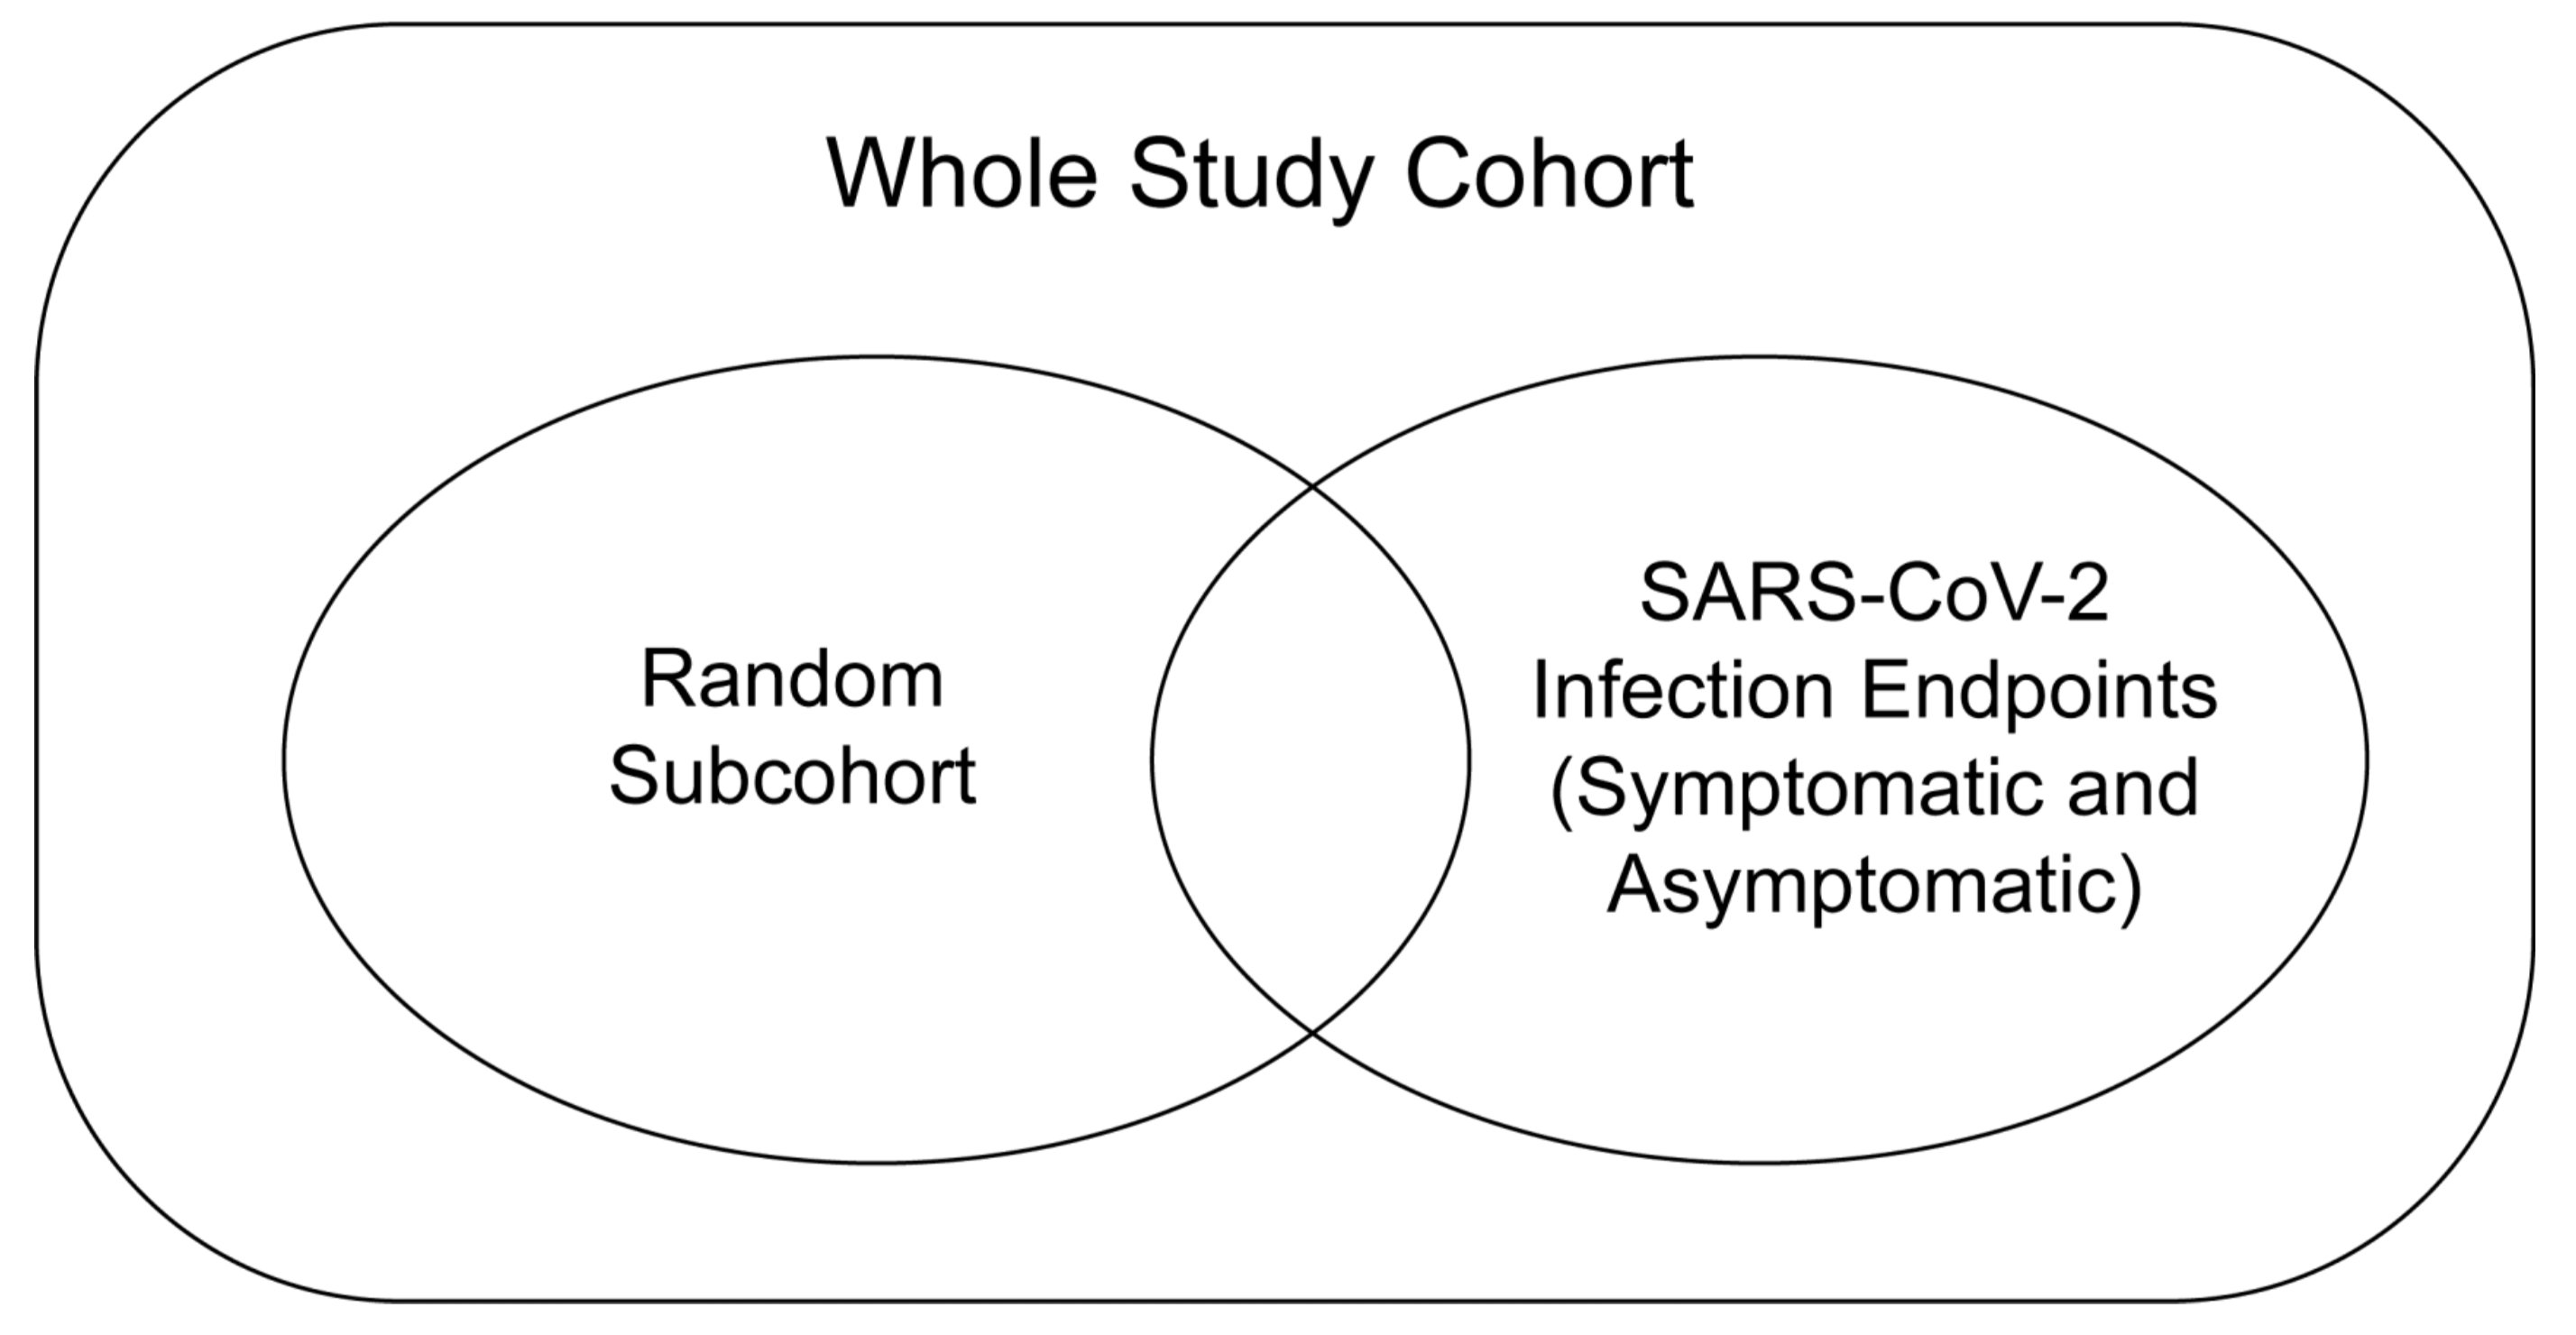
\includegraphics[scale=0.15]{casecohort}
  \captionsetup{labelformat=empty}
  \vspace{-1em}
  \caption{
    \tiny Case-cohort design, per~\citet{prentice1986case}, as applied to COVE.
  }
\end{figure}
\end{center}

\note{
}

\end{frame}

%%%%%%%%%%%%%%%%%%%%%%%%%%%%%%%%%%%%%%%%%%%%%%%%%%%%%%%%%%%%%%%%%%%%%%%%%%%%%%%%

%\begin{frame}[c]{A Simple Two-Phase Design: Case-Cohort}

%Assaying >30k samples is expensive, statistically unnecessary.
%\vspace{-1em}
%\begin{figure}[H]
  %\centering
  %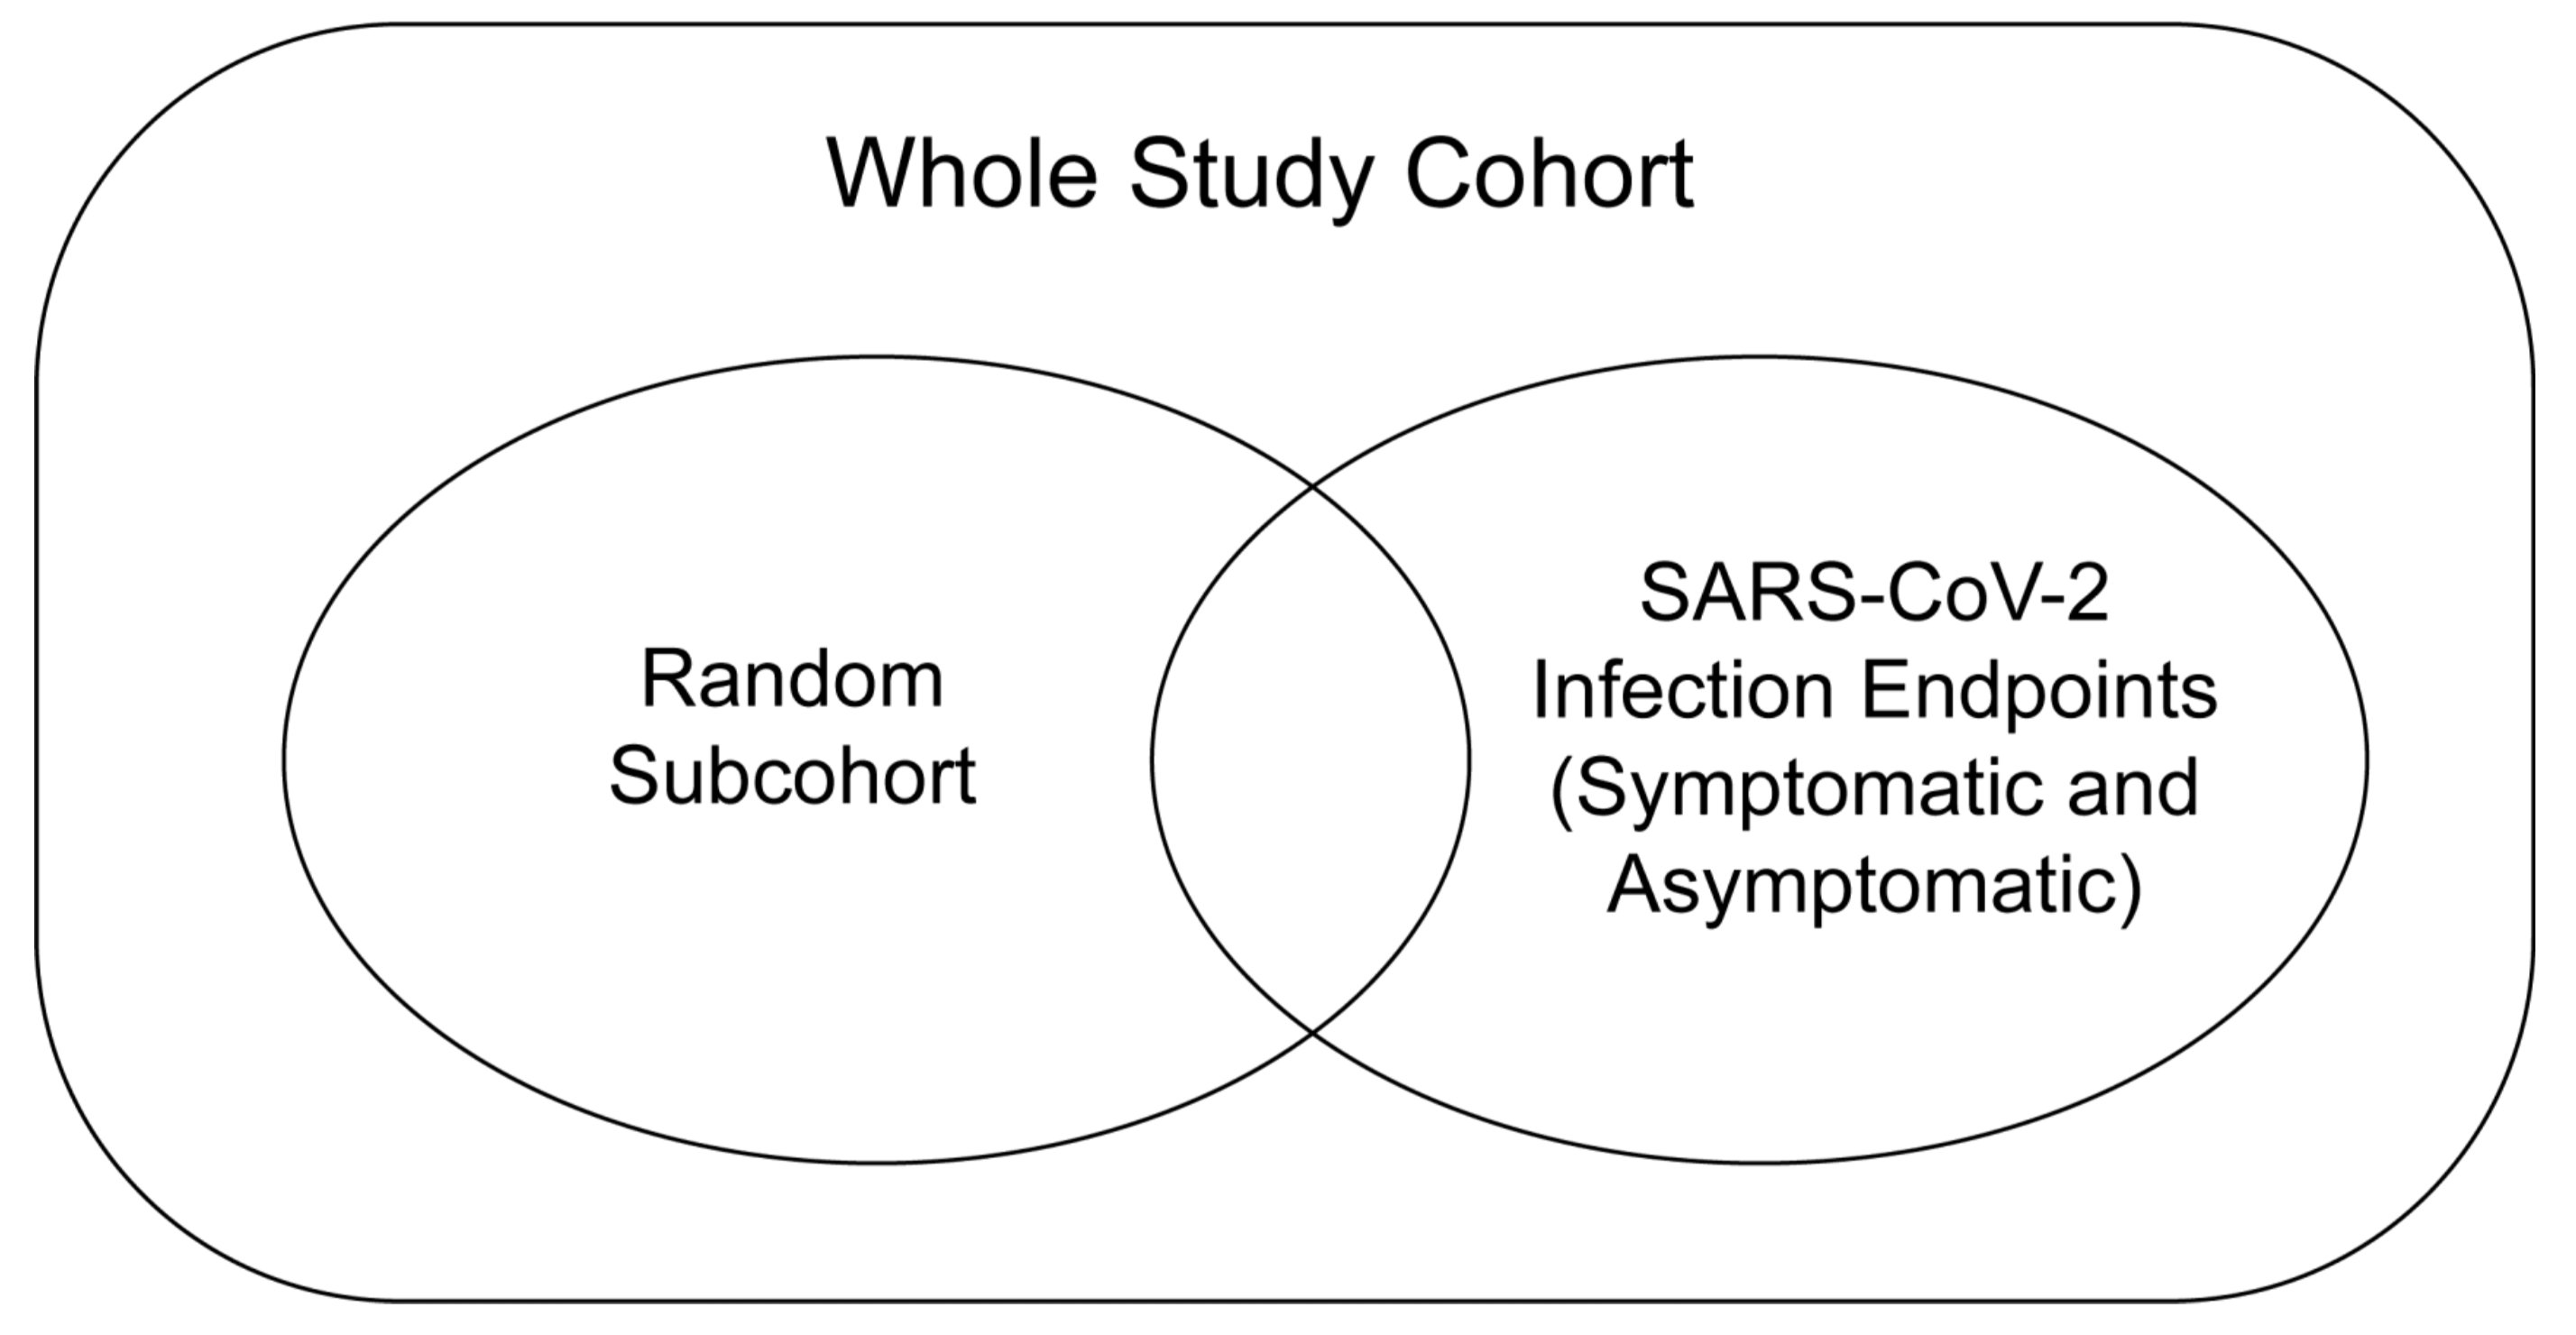
\includegraphics[scale=0.23]{casecohort}
  %\captionsetup{labelformat=empty}
  %\vspace{-1.5em}
  %\caption{
    %Case-cohort design, per~\citet{prentice1986case}, as applied to COVE.
  %}
%\end{figure}

%\note{
%}

%\end{frame}

%%%%%%%%%%%%%%%%%%%%%%%%%%%%%%%%%%%%%%%%%%%%%%%%%%%%%%%%%%%%%%%%%%%%%%%%%%%%%%%%

\begin{frame}[c]{Two-phase Sampling Masks the Complete Data Structure}

\begin{center}
\begin{itemize}
  \itemsep8pt
  \item Complete (unobserved) data $X = (L, A, S, Y) \sim P_{0,X} \in
    \mathcal{M}$:
    \begin{itemize}
      \itemsep4pt
      \item $L$ (baseline covariates): sex, age, BMI, behavioral HIV risk,
      \item $A$ (treatment): randomized assignment to vaccine/placebo,
      \item $S$ (mediator): immune response profile for a given marker,
      \item $Y$ (outcome of interest): infection status at trial's end.
    \end{itemize}
  \item Observed data $O = (B, BX) = (L, B, BS, Y) \sim P_0 \in \mathcal{M}$.
    \begin{itemize}
      \itemsep4pt
      \item $B \in \{0,1\}$ indicates inclusion in the second-phase sample.
      \item $\pi_0 \coloneqq \pr(B = 1 \mid Y, L)$ must be \textit{known by
        design} or estimated.
      \item Implicitly conditioning on the vaccine arm: $O = \{X \mid A = 1\}$.
    \end{itemize}
\end{itemize}
\end{center}

\note{
  \begin{itemize}
    \item $P_0^X$ --- true (unknown) distribution of the full data $X$.
    \item $\mathcal{M}$ --- nonparametric statistical model.
  \end{itemize}
}

\end{frame}

%%%%%%%%%%%%%%%%%%%%%%%%%%%%%%%%%%%%%%%%%%%%%%%%%%%%%%%%%%%%%%%%%%%%%%%%%%%%%%%%

%\begin{frame}[standout]
  %Causal Effects for Quantitative Exposures
%\end{frame}

%%%%%%%%%%%%%%%%%%%%%%%%%%%%%%%%%%%%%%%%%%%%%%%%%%%%%%%%%%%%%%%%%%%%%%%%%%%%%%%%

%\begin{frame}[c]{Static Interventions Aren't Enough}

%\begin{center}
%\begin{itemize}
  %\itemsep8pt
  %\item Describe the manner in which $X$ is hypothetically generated by a
    %nonparametric structural equation model~\citep{pearl2009causality}:
    %\begin{equation*}
      %L = f_L(U_L); A \sim \text{Bern}(0.5);
      %S = f_S(A, L, U_S); Y = f_Y(S, A, L, U_Y)
    %\end{equation*}
  %\item Implies a model for the distribution of counterfactual random variables
    %induced by interventions on the system.
  %\item A \textit{static} intervention replaces $f_S$ with a specific value $s$
    %in its conditional support $S \mid L$.
  %\item This requires specifying \textit{a priori} a particular value of
    %exposure under which to evaluate the outcome --- but what value?
%\end{itemize}
%\end{center}

%\note{
%}

%\end{frame}

%%%%%%%%%%%%%%%%%%%%%%%%%%%%%%%%%%%%%%%%%%%%%%%%%%%%%%%%%%%%%%%%%%%%%%%%%%%%%%%%

\begin{frame}[c]{Causal Effects of Modified Treatment Policies}

\begin{center}
\begin{itemize}
  \itemsep8pt
  \item Stochastic interventions modify the value $S$ would naturally assume by
    \textit{shifting} the natural exposure distribution.
  \item \cite{diaz2012population, diaz2018stochastic}'s shift
    interventions\footnotemark
    \begin{equation*}\label{shift_intervention}
      d(s, l; \delta) =
        \begin{cases}
          s + \delta, & s + \delta < u(l) \quad (\text{if plausible}) \\
          s, & s + \delta \geq u(l) \quad (\text{otherwise})
        \end{cases}
    \end{equation*}
  %\item Our estimand, $\psi_{0,\delta} \coloneqq
    %\E_{P_{0, \delta}}\{Y(d(S,L;\delta))\}$, is identified by
    %\begin{align*}\label{eqn:identification2012}
      %\psi_{0,\delta} = \int_{\mathcal{L}} \int_{\mathcal{S}} &\E_{P_0}
        %\{Y \mid S = d(s, l; \delta), L = l\} \\ &g_{0, S}(s \mid L = l)
        %q_{0, L}(l) d\mu(s)d\nu(l)
    %\end{align*}
  \item Our estimand, $\psi_{0,\delta} \coloneqq
    \E_{P_{0, \delta}}\{Y(d(S,L;\delta))\}$ is \textit{counterfactual mean}
    risk when the distribution of $S$ is shifted by $\delta$ units.
\end{itemize}
\end{center}

\note{
}

\footnotetext[1]{\citet{haneuse2013estimation} introduced modified treatment
policies.}

\end{frame}

%%%%%%%%%%%%%%%%%%%%%%%%%%%%%%%%%%%%%%%%%%%%%%%%%%%%%%%%%%%%%%%%%%%%%%%%%%%%%%%%

\begin{frame}[c]{Disease Risk Under Shifted Immunogenic Responses}

\hspace*{-1cm}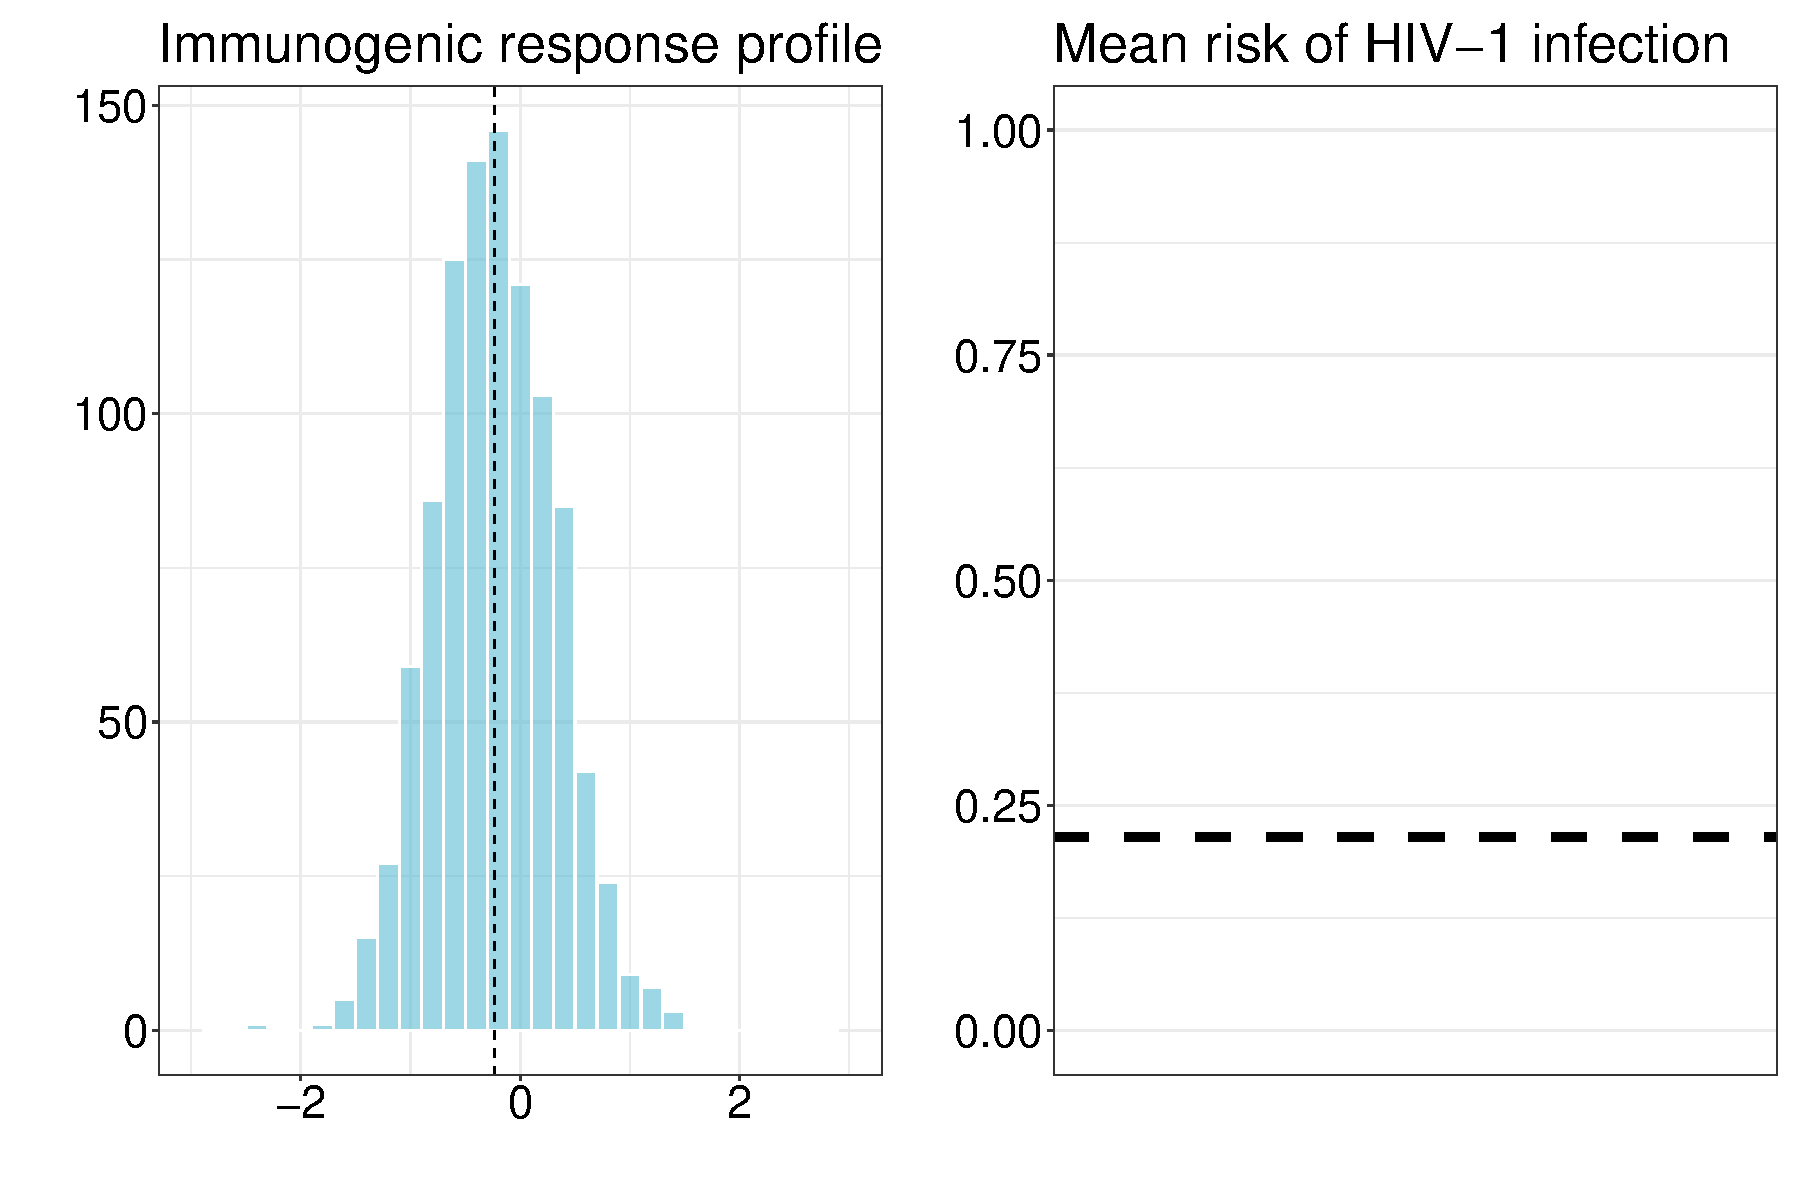
\includegraphics[scale=0.41]{shift-5}

\note{
}

\end{frame}

%%%%%%%%%%%%%%%%%%%%%%%%%%%%%%%%%%%%%%%%%%%%%%%%%%%%%%%%%%%%%%%%%%%%%%%%%%%%%%%%

\begin{frame}[c]{Disease Risk Under Shifted Immunogenic Responses}

\hspace*{-1cm}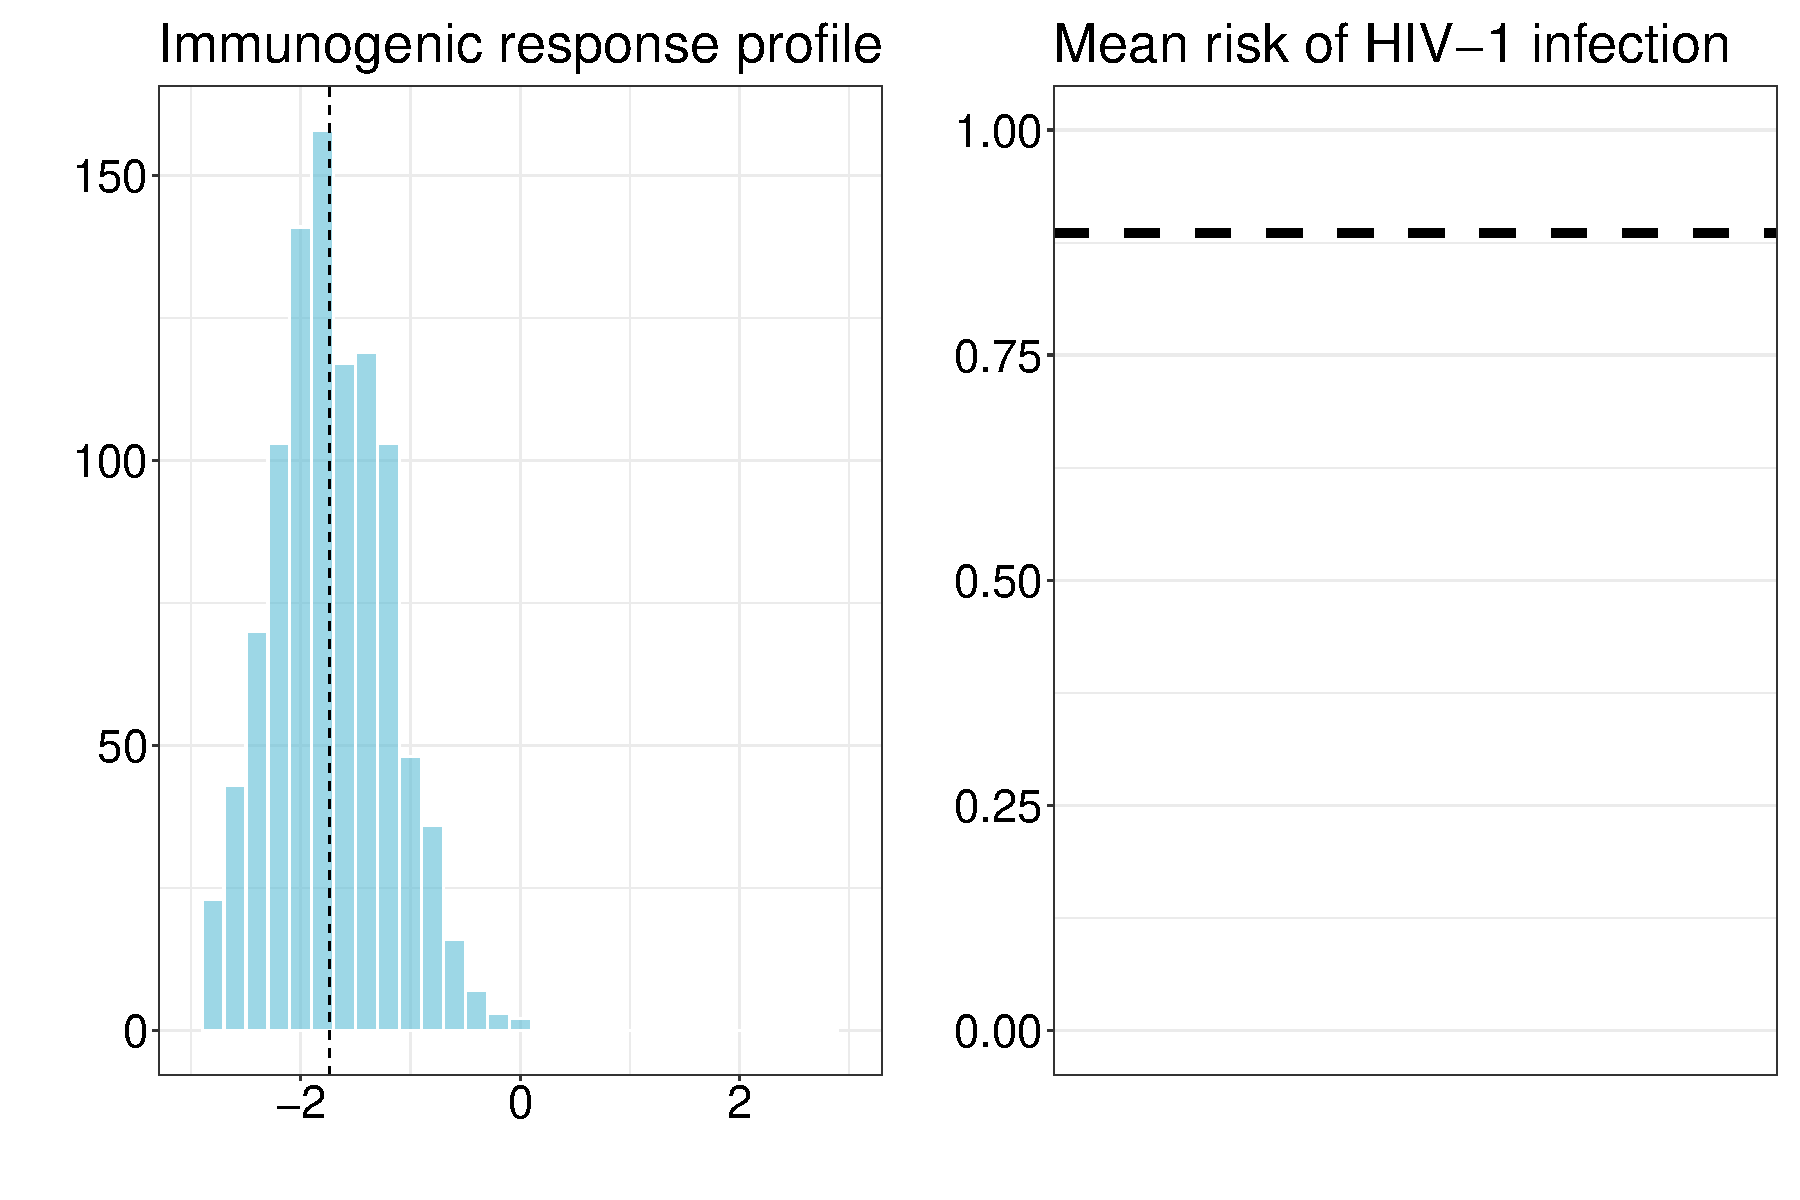
\includegraphics[scale=0.41]{shift-2}

\note{
}

\end{frame}

%%%%%%%%%%%%%%%%%%%%%%%%%%%%%%%%%%%%%%%%%%%%%%%%%%%%%%%%%%%%%%%%%%%%%%%%%%%%%%%%

\begin{frame}[c]{Disease Risk Under Shifted Immunogenic Responses}

\hspace*{-1cm}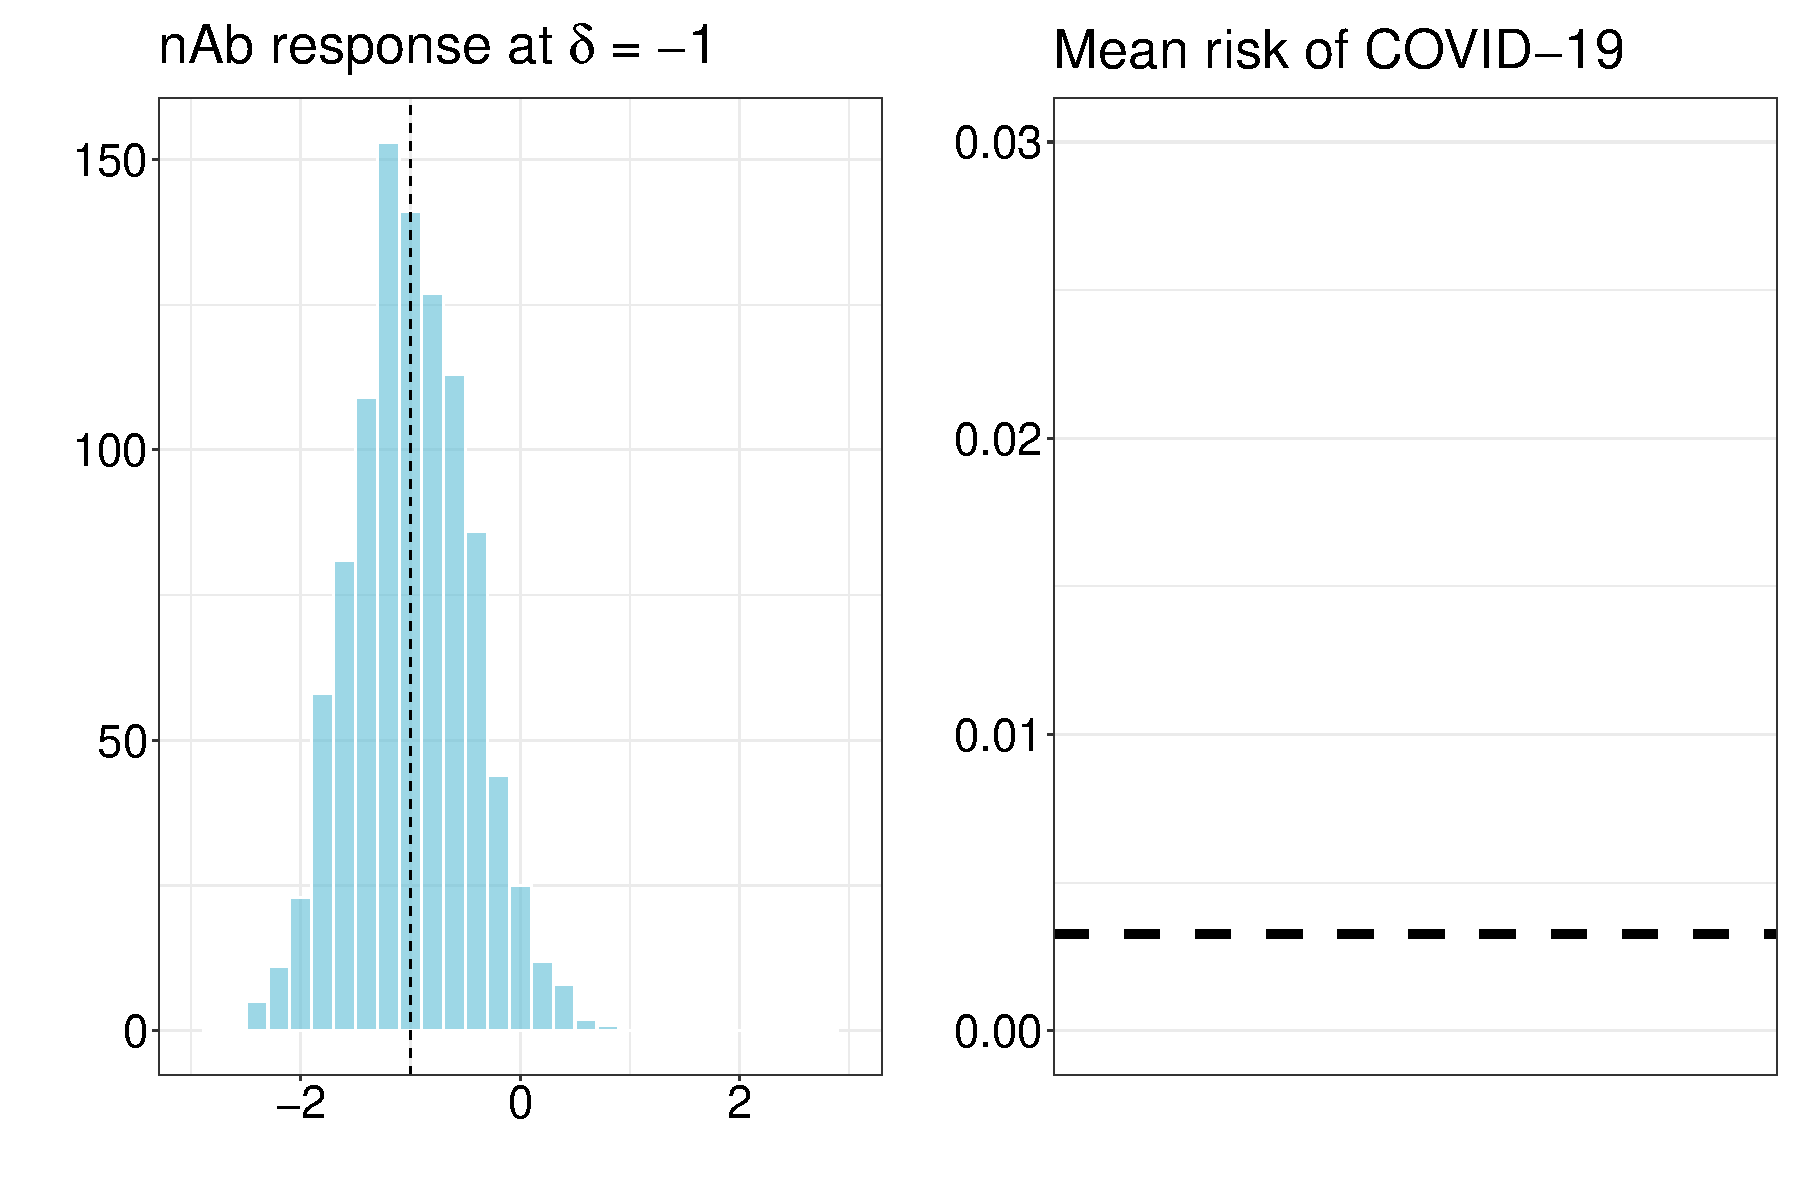
\includegraphics[scale=0.41]{shift-3}

\note{
}

\end{frame}

%%%%%%%%%%%%%%%%%%%%%%%%%%%%%%%%%%%%%%%%%%%%%%%%%%%%%%%%%%%%%%%%%%%%%%%%%%%%%%%%

\begin{frame}[c]{Disease Risk Under Shifted Immunogenic Responses}

\hspace*{-1cm}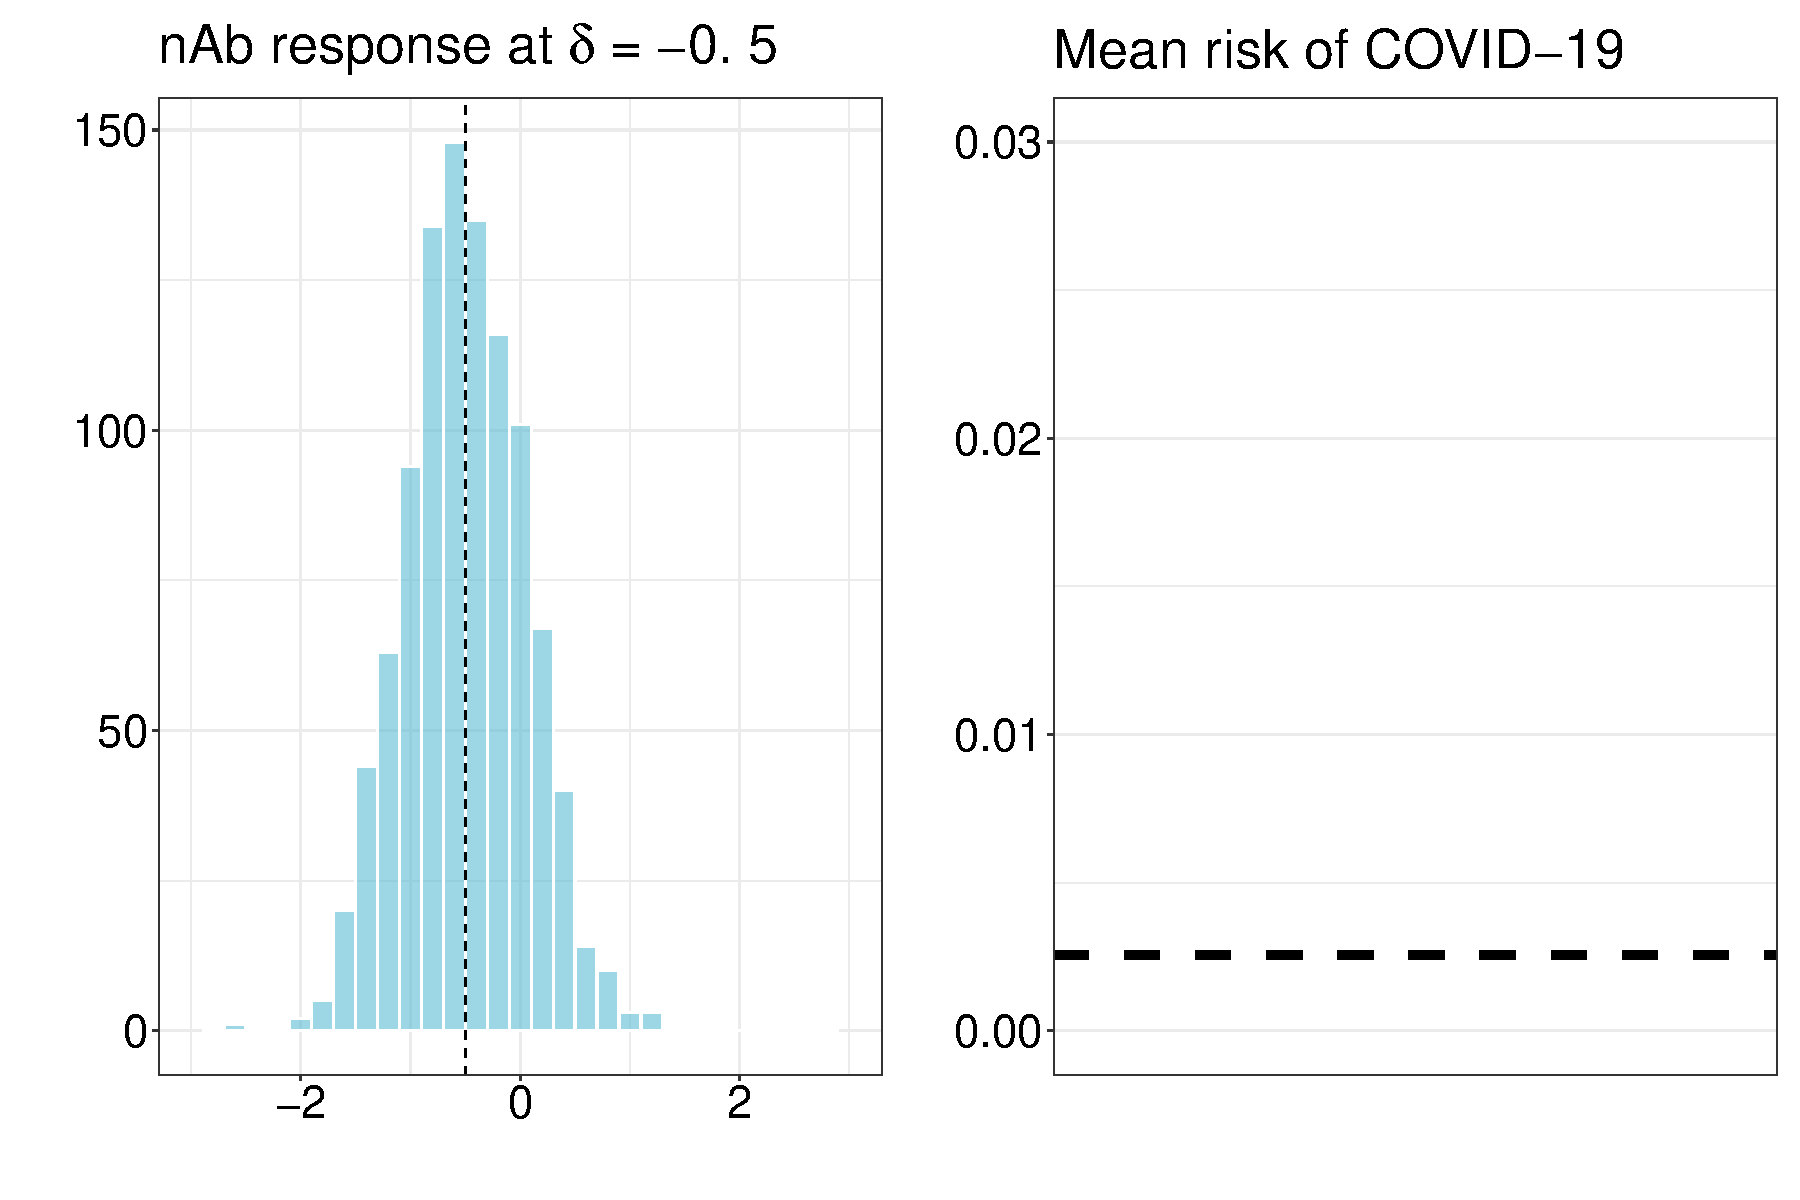
\includegraphics[scale=0.41]{shift-4}

\note{
}

\end{frame}

%%%%%%%%%%%%%%%%%%%%%%%%%%%%%%%%%%%%%%%%%%%%%%%%%%%%%%%%%%%%%%%%%%%%%%%%%%%%%%%%

\begin{frame}[c]{Disease Risk Under Shifted Immunogenic Responses}

\hspace*{-1cm}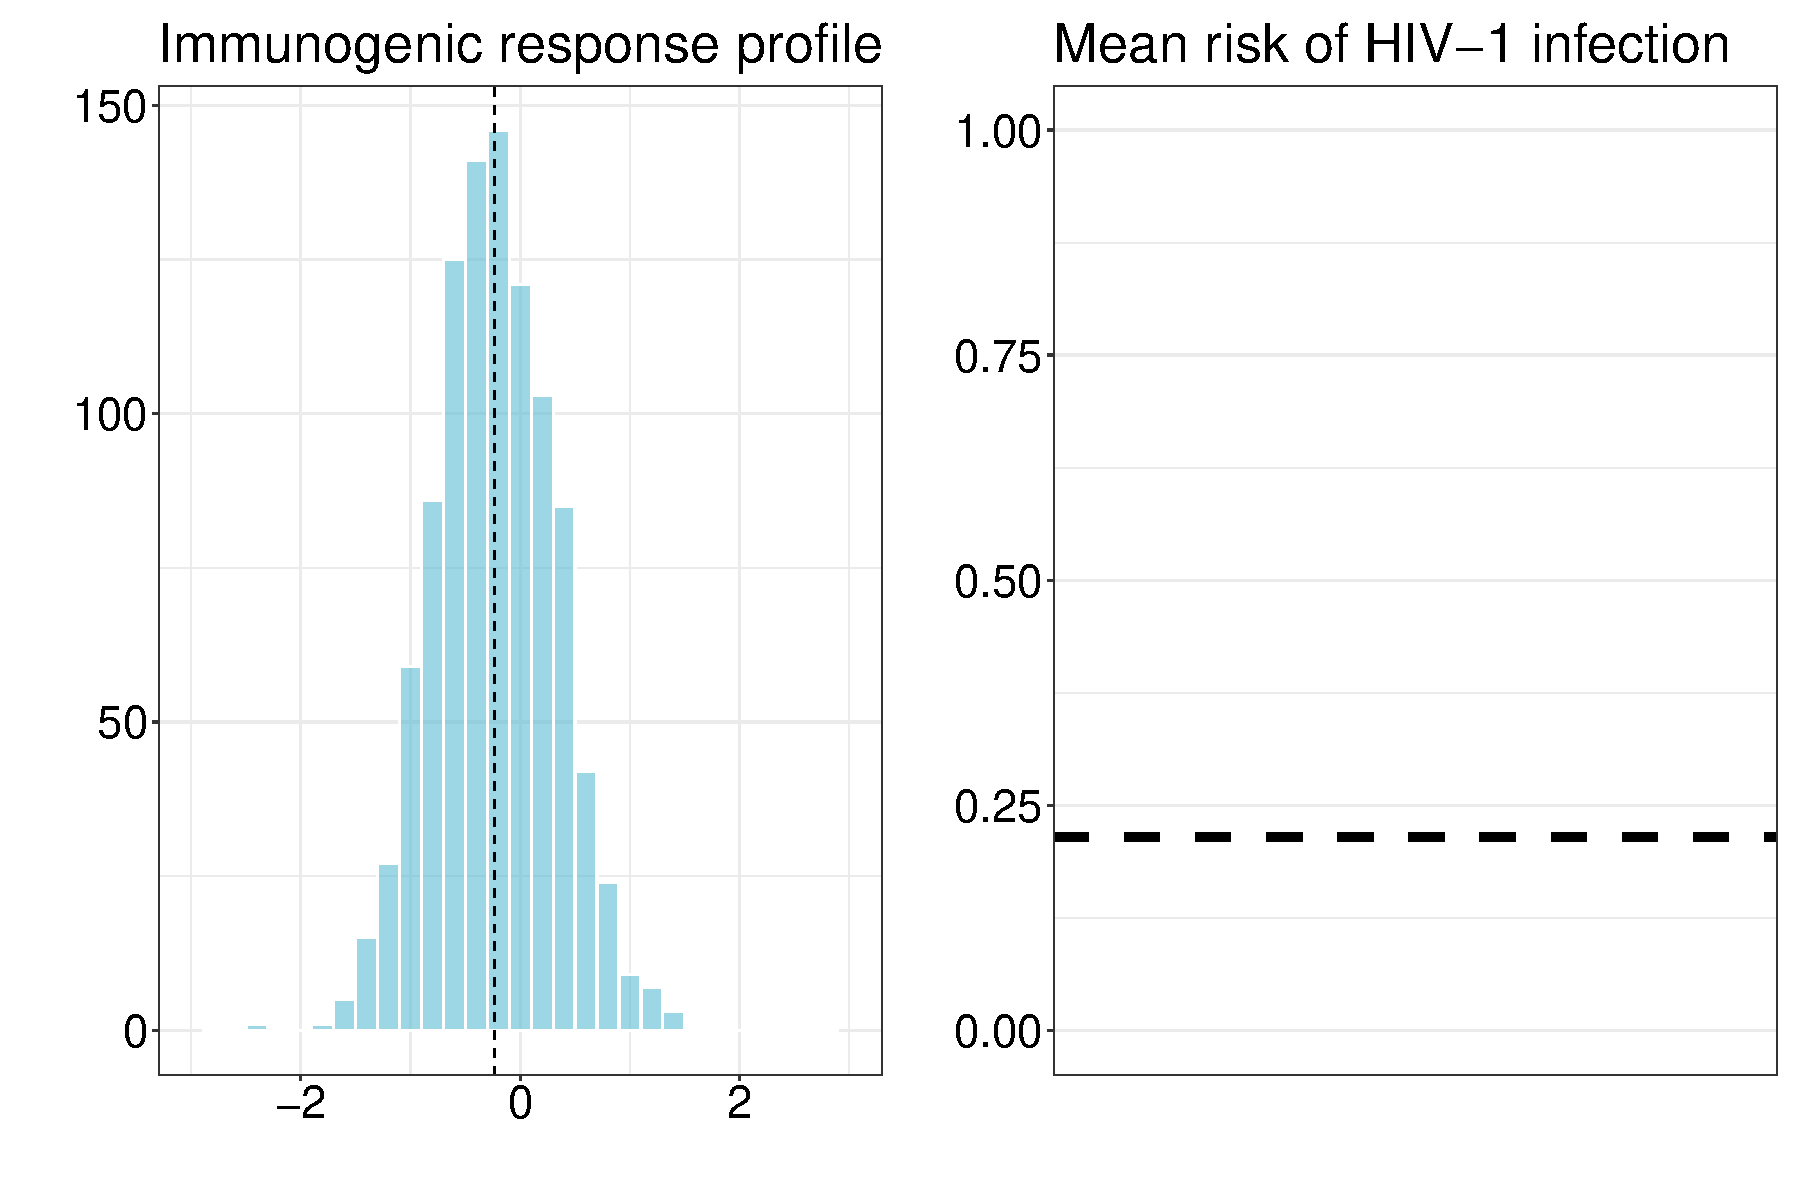
\includegraphics[scale=0.41]{shift-5}

\note{
}

\end{frame}

%%%%%%%%%%%%%%%%%%%%%%%%%%%%%%%%%%%%%%%%%%%%%%%%%%%%%%%%%%%%%%%%%%%%%%%%%%%%%%%%

%\begin{frame}[c]{Interpreting the Causal Effects of Shift Interventions}

%\begin{center}
%\begin{itemize}
  %\itemsep6pt
  %\item Consider a data structure: $(Y_s, s \in \mathcal{S})$.
  %\item Let $Y_s = \beta_0 + \beta_1 s + \epsilon_s$, with error $\epsilon_s
    %\sim N(0, \sigma^2_s)$ $\forall s \in S$.
  %\item For the counterfactual outcomes $(Y_{s' + \delta}, Y_{s'})$, their
    %difference $Y_{s' + \delta} - Y_{s'}$ may be expressed (for some
    %$s' \in \mathcal{S}$)
    %\begin{align*}
      %\E Y_{s' + \delta} - \E Y_{s'} &= [\beta_0 + \beta_1 (s' + \delta) +
          %\E \epsilon_{s' + \delta}] - [\beta_0 + \beta_1 s' +
          %\E \epsilon_{s'}] \\
        %&= \beta_1 \delta
    %\end{align*}
  %\item A \textit{unit shift} for $s' \in S$ (i.e., $\delta = 1$) causes a
    %counterfactual difference in $Y$ of magnitude $\beta_1$.
%\end{itemize}
%\end{center}

%\note{
  %\begin{itemize}
    %\item Note that this analysis is exactly what we're told we \textbf{cannot}
      %do in ``linear models 101'' --- that is, the slope of a regression line
      %cannot be interpreted as \textit{causing} a change in the outcome.
    %\item We extend this result to the mean counterfactual outcomes under the
      %nonparametric model $\M$.
  %\end{itemize}
%}

%\end{frame}

%%%%%%%%%%%%%%%%%%%%%%%%%%%%%%%%%%%%%%%%%%%%%%%%%%%%%%%%%%%%%%%%%%%%%%%%%%%%%%%%

%\begin{frame}[c]{Stochastic--Interventional Vaccine Efficacy}

%\begin{center}
%\begin{itemize}
  %\itemsep8pt
  %\item Causal parameter based on vaccine efficacy (VE) estimands:
  %\begin{align*}
    %\text{SVE}(\delta) &= 1 - \frac{\E[\pr(Y = 1 \mid S = d(s, l), A = 1,
                                    %L = l)]}{\pr(Y(0)=1)} \\
                       %&= 1 - \frac{\psi_{0, \delta}}{\pr(Y(0)=1)}
  %\end{align*}
  %\item $\pr(Y(0)=1)$: counterfactual infection risk in the placebo arm ---
    %under randomization, $\pr(Y(0)=1) \equiv \pr(Y=1 \mid A=0)$.
  %\item Summarizes VE via stochastic interventions across $\delta$, per the
    %CoVPN immune correlates SAP\footnotemark~\citep{gilbert2021covpn,
    %gilbert2021immune}.
%\end{itemize}
%\end{center}

%\note{
%}

%\footnotetext[2]{SAP published at
%\url{https://doi.org/10.6084/m9.figshare.13198595}.}

%\end{frame}

%%%%%%%%%%%%%%%%%%%%%%%%%%%%%%%%%%%%%%%%%%%%%%%%%%%%%%%%%%%%%%%%%%%%%%%%%%%%%%%%

%\begin{frame}[standout]
  %Efficient Estimation in Two-Phase Designs
%\end{frame}

%%%%%%%%%%%%%%%%%%%%%%%%%%%%%%%%%%%%%%%%%%%%%%%%%%%%%%%%%%%%%%%%%%%%%%%%%%%%%%%

%\begin{frame}{Estimation of the Counterfactual Mean $\psi_{0,\delta}$}
%An \textit{estimator} $\psi_{n,\delta}$ of $\psi_{0,\delta} \coloneqq \Psi(P_0)$
%is \textit{efficient} if and only if
%\[
  %\psi_{n,\delta} - \psi_{0, \delta} = n^{-1} \sum\limits_{i=1}^n
  %D^{\star}(P_0)(O_i) + o_P(n^{-1/2}) \ ,
%\]
%where $D^{\star}(P)$ is the \textit{efficient influence function} (EIF) of
%$\psi_{0,\delta}$ with respect to the nonparametric model $\mathcal{M}$ at a
%distribution $P$.
%\vspace{0.25cm}

%The EIF of $\psi_{0,\delta}$ is indexed by two key \textit{nuisance parameters}
%\begin{align*}
  %\overline{Q}_{Y}(S,L) &\coloneqq \E_{P}(Y \mid S, L) &
      %\mbox{\textit{outcome mechanism}} \\
  %g_{S}(S \mid L) &\coloneqq p(S \mid L) &
    %\mbox{\textit{generalized propensity score}}
%\end{align*}

%\note{
%}

%\end{frame}

%%%%%%%%%%%%%%%%%%%%%%%%%%%%%%%%%%%%%%%%%%%%%%%%%%%%%%%%%%%%%%%%%%%%%%%%%%%%%%%%

\begin{frame}[c]{Flexible, Efficient, Robust Estimation}

\begin{center}
\begin{itemize}
  \itemsep8pt
  \item The efficient influence function $D^{\star}(P)(O_i)$ of
    $\psi_{0, \delta}$ wrt $\mathcal{M}$ is a critical ingredient for
    constructing \textit{efficient} estimators.
    %\begin{equation*}
      %D^{\star}_{F}(P_0)(o) = \frac{g_{0,S}(d^{-1}(s,l) \mid l)}
      %{g_{0,S}(s \mid l)} ({y - \overline{Q}_{0,Y}(s,l)}) +
      %\overline{Q}_{0,Y}(d(s,l), l) - \psi_{0,\delta}.
    %\end{equation*}
  \item One-step estimator $\psi_n^{+}$ performs an additive bias-correcting
    update ``directly'' in parameter space.
    %\begin{equation*}\label{tmle}
        %\psi_n^{+} = \frac{1}{n} \sum_{i = 1}^n \overline{Q}_{n,Y}(d(S_i, L_i),
        %L_i) + D^{\star}_n(O_i).
      %\end{equation*}
  \item The TML estimator $\psi_n^{\star}$ performs a bias-correcting update in
    model space by way of (parametric) tilting/fluctuation.
    %\begin{equation*}\label{tmle}
      %\psi_n^{\star} = \frac{1}{n} \sum_{i = 1}^n
      %\overline{Q}_{n,Y}^{\star}(d(S_i, L_i), L_i).
    %\end{equation*}
  \item Both doubly robust: \textit{machine learning} for nuisance estimation!
  \item Still, must \textbf{correct for} two-phase sampling bias --- but how?
\end{itemize}
\end{center}

\note{
  \begin{itemize}
    \item Both estimators are CAN even when nuisance parameters are estimated
      via flexible, machine learning techniques.
    \item Semiparametric-efficient estimation thru solving efficient influence
      function estimating equation wrt the model $\M$.
    \item The auxiliary covariate simplifies when the treatment is in the limits
      (conditional on $W$) --- i.e., for $S_i \in (u(l) - \delta, u(l))$, then
      we have $H(s,l) = \frac{g_0(s - \delta \mid l)}{g_0(s \mid l)} + 1$.
    \item Need to explicitly remind the audience what $u(l)$ is again. It's only
      appeared once at this point, and only been mentioned in passing.
  \end{itemize}
}

\end{frame}

%%%%%%%%%%%%%%%%%%%%%%%%%%%%%%%%%%%%%%%%%%%%%%%%%%%%%%%%%%%%%%%%%%%%%%%%%%%%%%%%

%\begin{frame}[c]{Augmented Estimators for Two-Phase Sampling Designs}

%\begin{center}
%\begin{itemize}
  %\itemsep8pt
  %\item \cite{rose2011targeted2sd} suggested inverse probability of censoring
    %weighted (IPCW) loss functions:
    %\begin{equation*}
      %\lik(P_0^X)(O) = \frac{B}{\pi_0(Y, L)}\lik(P_0^X)(X)
    %\end{equation*}
  %\item When the sampling mechanism $\pi_0(Y,L)$ is known by design, this
    %procedure yields a reasonably reliable estimator.
  %\item When data-adaptive regression must be used --- that is, when
    %$\pi_0(Y,L)$ is not known by design\footnotemark --- this is insufficient.
%\end{itemize}
%\end{center}

%\note{
%}

%\footnotetext[3]{Sampling of non-cases in HVTN 505 used
%matching~\citep{janes2017higher}.}

%\end{frame}

%%%%%%%%%%%%%%%%%%%%%%%%%%%%%%%%%%%%%%%%%%%%%%%%%%%%%%%%%%%%%%%%%%%%%%%%%%%%%%%%

%\begin{frame}[c]{Efficiency and Multiple Robustness~\citep{hejazi2020efficient}}

%\begin{center}
%\begin{itemize}
  %\itemsep8pt
  %\item Then, the IPCW augmentation must be applied to the EIF\footnotemark:
    %\begin{align*}
      %D^{\star}(P_0^X)(o) = &\frac{b}{\pi_0(y, l)} D^{\star}_F(P_0^X)(x) -
        %\left(1 - \frac{b}{\pi_0(y, l)}\right) \\
        %&\E(D^{\star}_F(P_0^X)(x) \mid B = 1, Y = y, L = l).
    %\end{align*}
  %\item Expresses observed data EIF $D^{\star}(P_0^X)(o)$ via complete data
     %EIF $D^{\star}_F(P_0^X)(x)$; inclusion of second term improves efficiency.
 %\item An emergent multiple robustness property --- combinations of
    %$\{g_0(S \mid L), \overline{Q}_0(S,L)\} \times \{\pi_0(Y, L),
    %\E(D^{\star}_F(P^X_0)(x) \mid B = 1, Y, L)\}$.
  %\item Our \texttt{txshift} \texttt{R} package implements our estimators of
    %$\psi_{0,\delta}$.
%\end{itemize}
%\end{center}

%\note{
%\begin{itemize}
  %\itemsep6pt
  %\item The expectation of the full data EIF $D^{\star}_F(P_0^X)(x)$, taken
    %only over units selected by the sampling mechanism (i.e., $B = 1$).
%\end{itemize}
%}

%\footnotetext[4]{A very general version appears to have been presented
%in~\citet{robins1994estimation}.}

%\end{frame}

%%%%%%%%%%%%%%%%%%%%%%%%%%%%%%%%%%%%%%%%%%%%%%%%%%%%%%%%%%%%%%%%%%%%%%%%%%%%%%%%


%\begin{frame}[c]{Comparing Reweighted and Augmented Estimators}

%\hspace*{-0.75cm}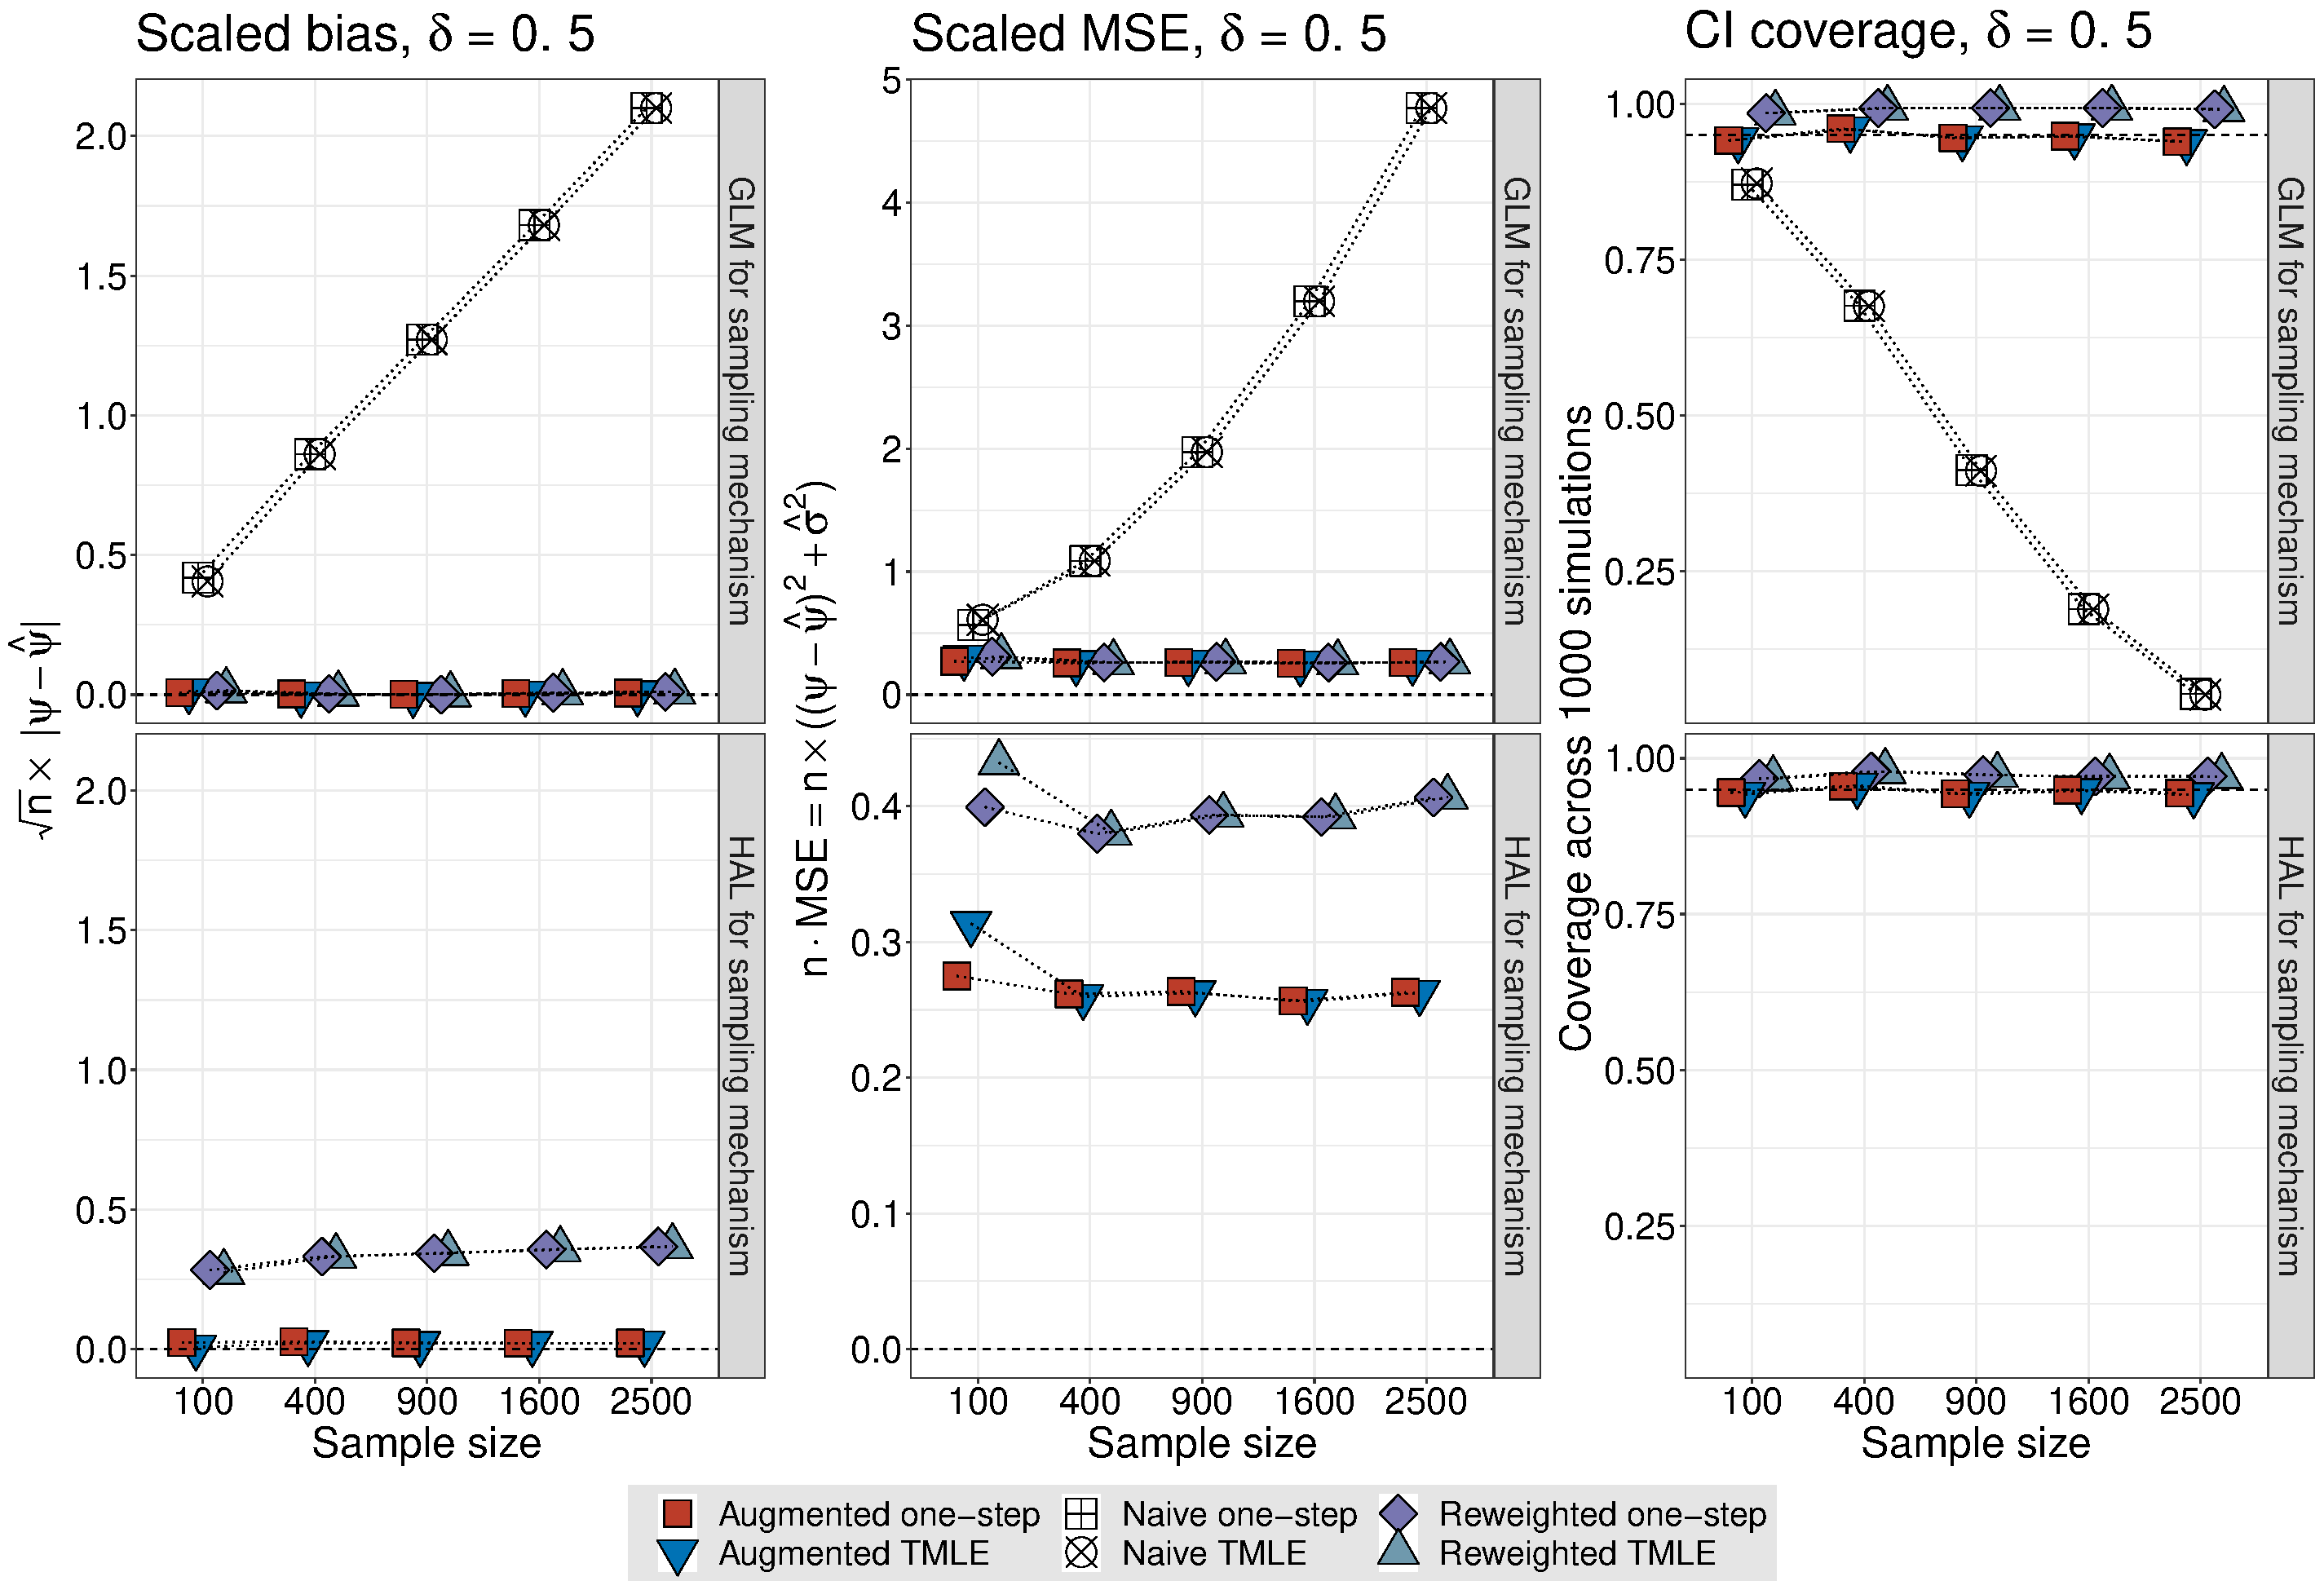
\includegraphics[scale=0.255]{simple_effect_panel_delta_upshift}

%\note{
%}

%\end{frame}

%%%%%%%%%%%%%%%%%%%%%%%%%%%%%%%%%%%%%%%%%%%%%%%%%%%%%%%%%%%%%%%%%%%%%%%%%%%%%%%%

%\begin{frame}[c]{SVE Prediction of HIV-1 Risk thru CD8+ Immune Response}

%\vspace{-0.3in}
%\begin{figure}[H]
  %\centering
  %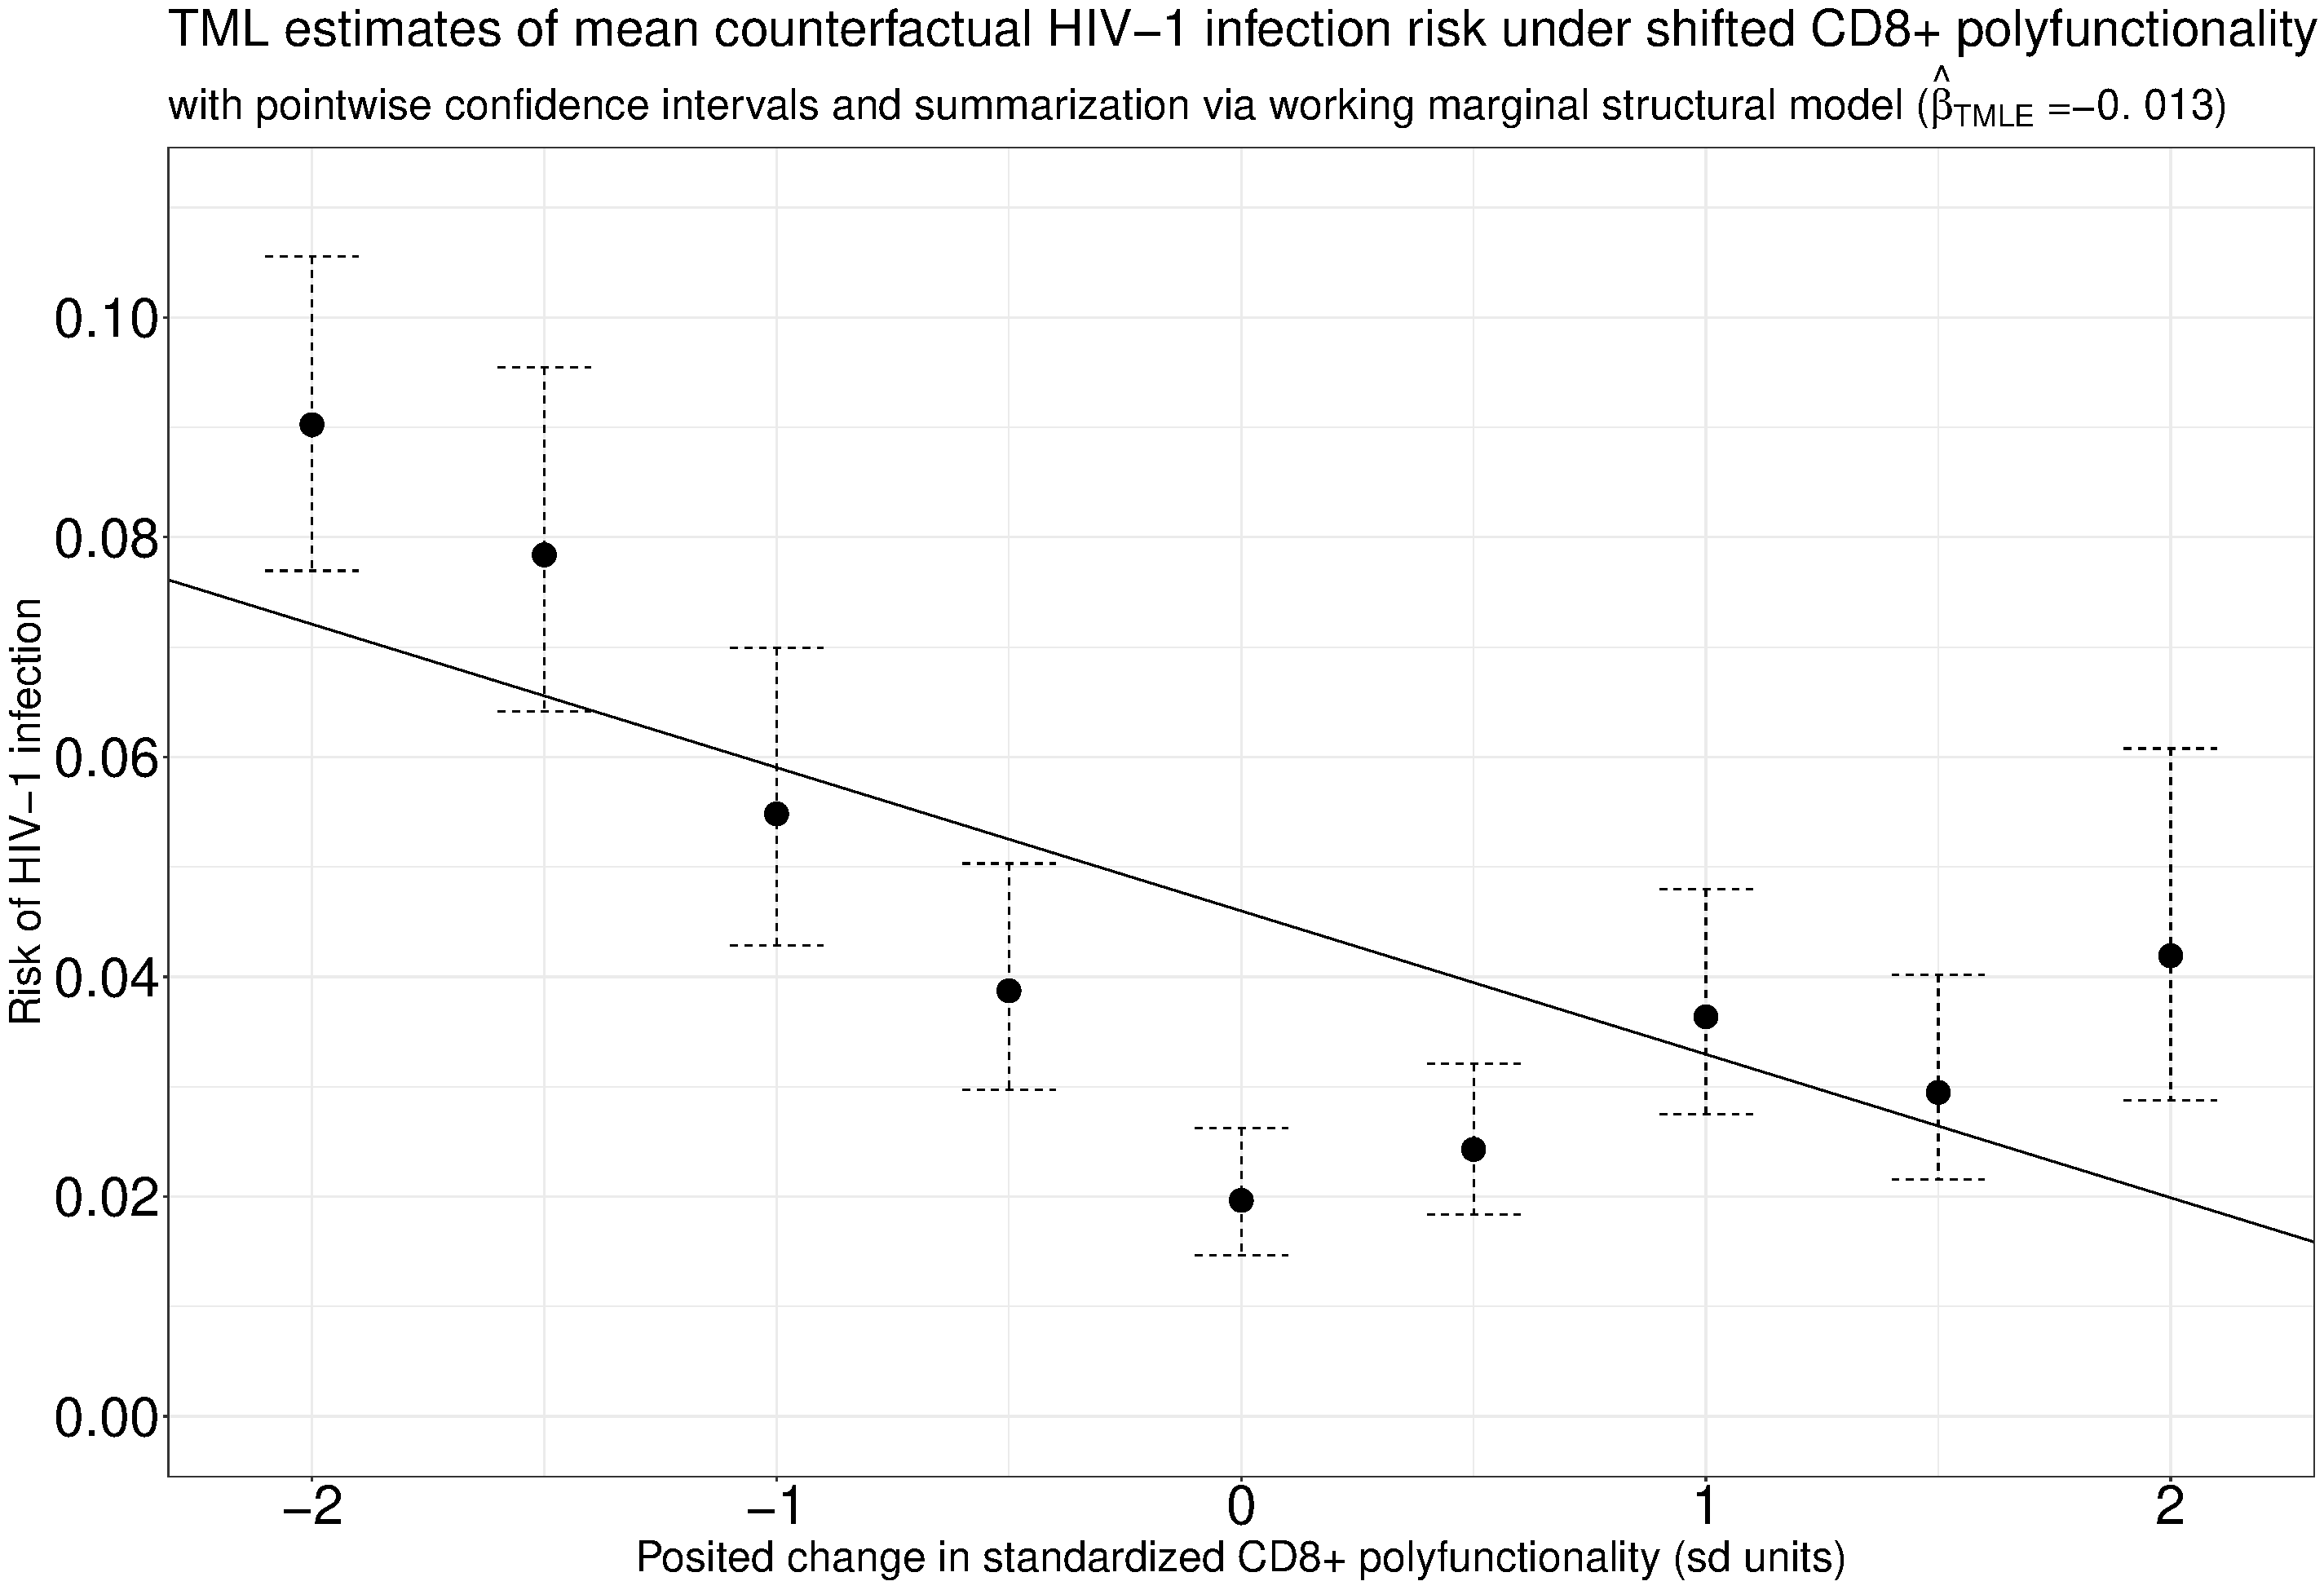
\includegraphics[scale=0.235]{cd8_msm_tmle_summary}
  %\captionsetup{labelformat=empty}
  %\vspace{-1.5em}
  %\caption{
    %HIV-1 risk change across CD8+ response (\texttt{txshift} \texttt{R}
    %package).
  %}
%\end{figure}

%\note{
%}

%\end{frame}

%%%%%%%%%%%%%%%%%%%%%%%%%%%%%%%%%%%%%%%%%%%%%%%%%%%%%%%%%%%%%%%%%%%%%%%%%%%%%%%%

\begin{frame}[c]{Prediction of mRNA-1273 VE thru PsV nAb Correlate}

\vspace*{-0.1cm}
\hspace*{-0.3cm}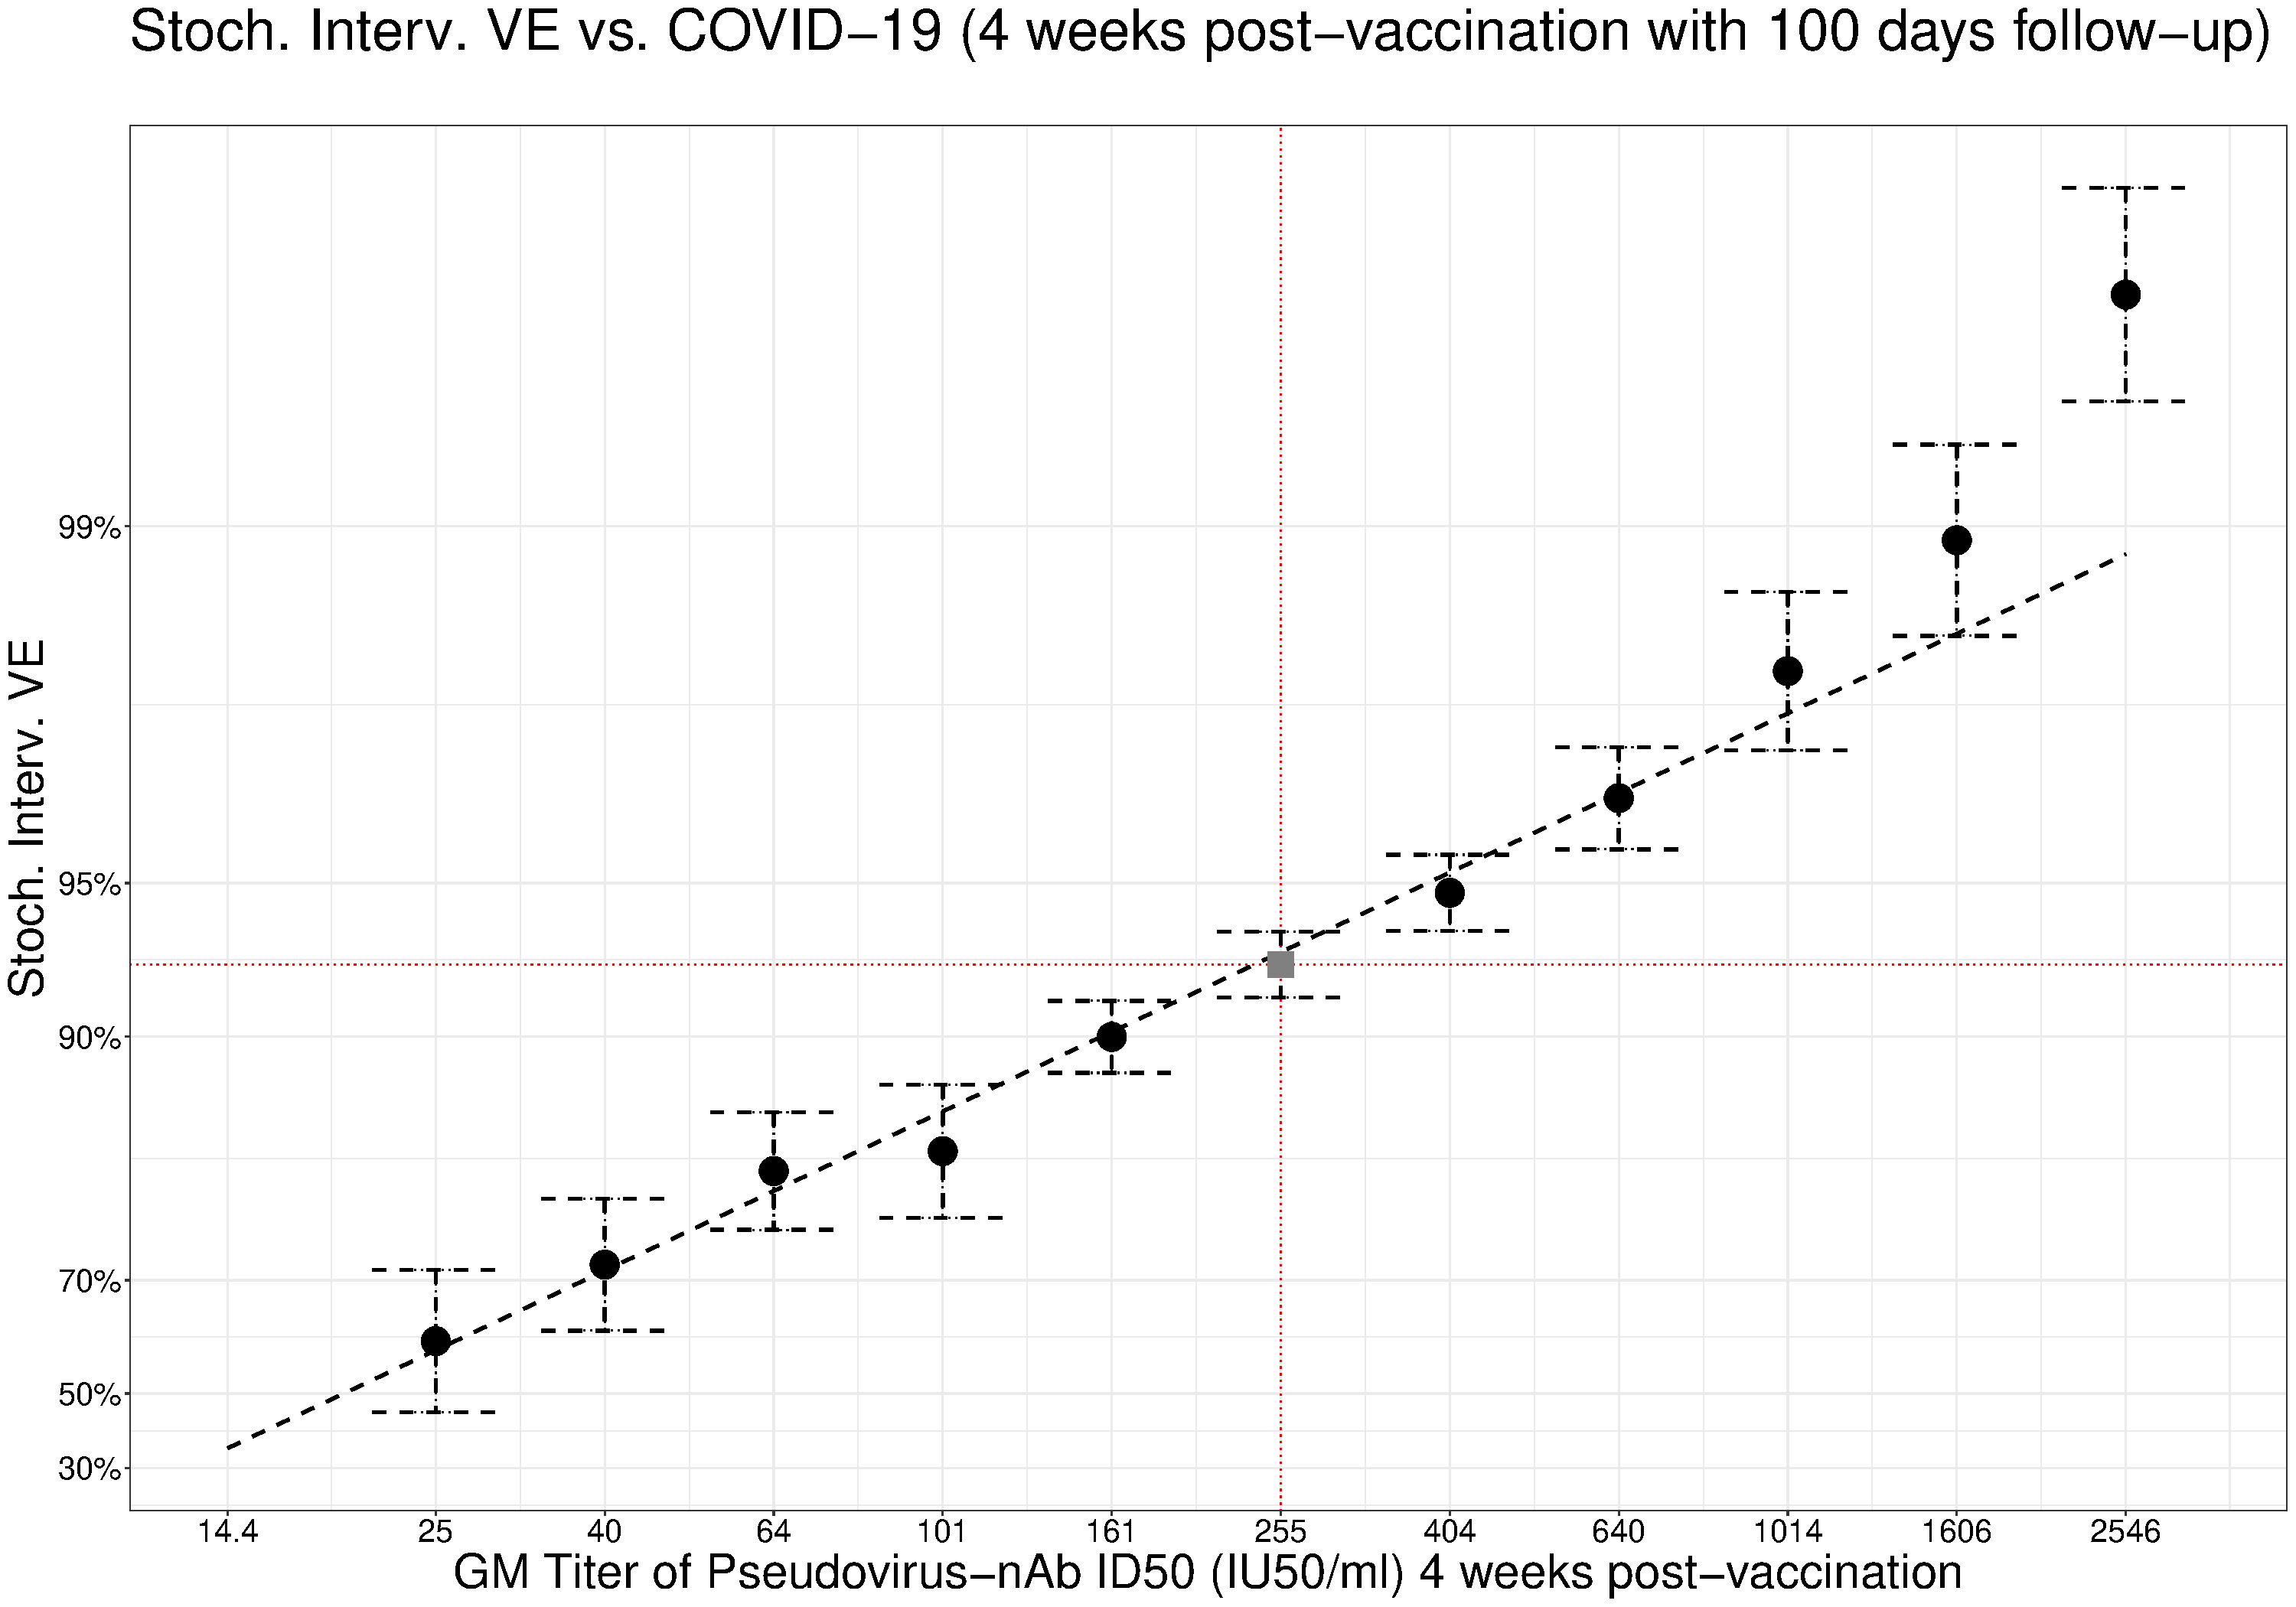
\includegraphics[scale=0.21]{sve_pseudoneutid50_simplified}

\note{
}

\end{frame}

%%%%%%%%%%%%%%%%%%%%%%%%%%%%%%%%%%%%%%%%%%%%%%%%%%%%%%%%%%%%%%%%%%%%%%%%%%%%%%%

%\begin{frame}[standout]
  %Bridging VE Using Immune Correlates
%\end{frame}

%%%%%%%%%%%%%%%%%%%%%%%%%%%%%%%%%%%%%%%%%%%%%%%%%%%%%%%%%%%%%%%%%%%%%%%%%%%%%%%%

%\begin{frame}[c]{Pooled Phase 1 Studies: PsV nAb Responses Across Variants}

%\vspace*{0.15cm}
%\hspace*{-0.8cm}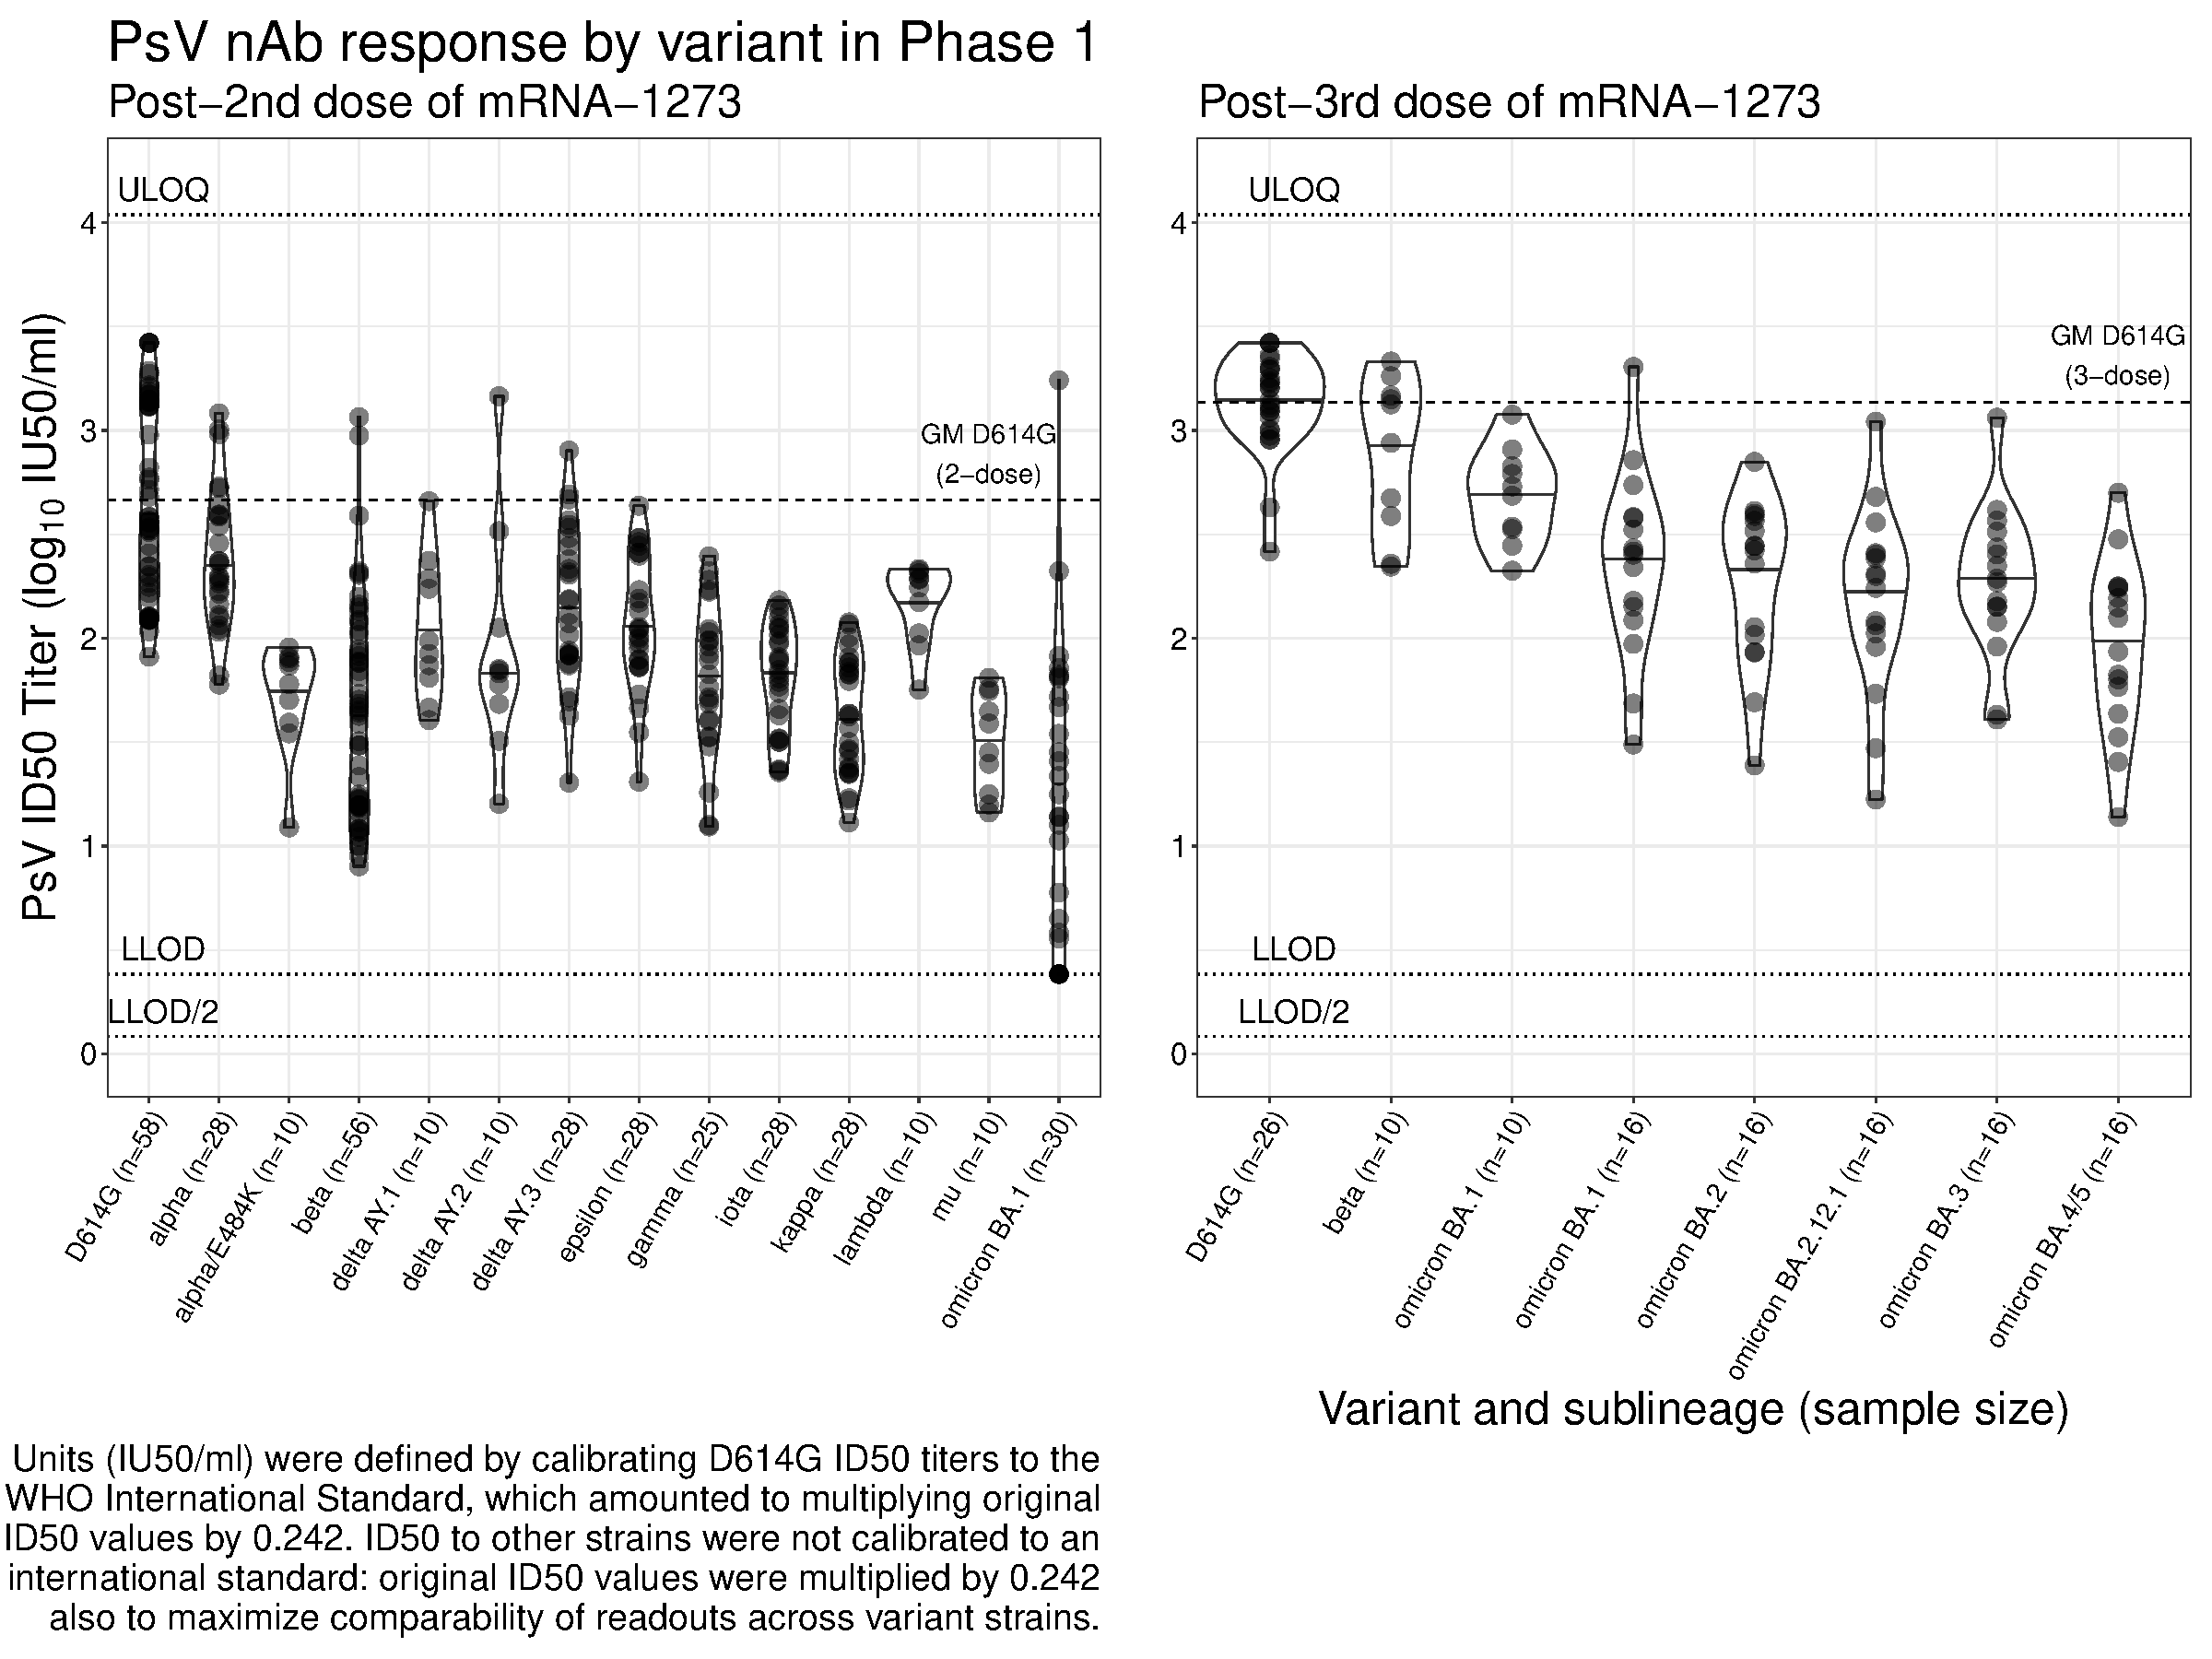
\includegraphics[scale=0.31]{variant_id50_eda}

%\note{
%}

%\end{frame}

%%%%%%%%%%%%%%%%%%%%%%%%%%%%%%%%%%%%%%%%%%%%%%%%%%%%%%%%%%%%%%%%%%%%%%%%%%%%%%%%

\begin{frame}[c]{Bridging of mRNA-1273 VE thru PsV nAb Correlate}

\vspace*{-0.1cm}
\hspace*{-0.3cm}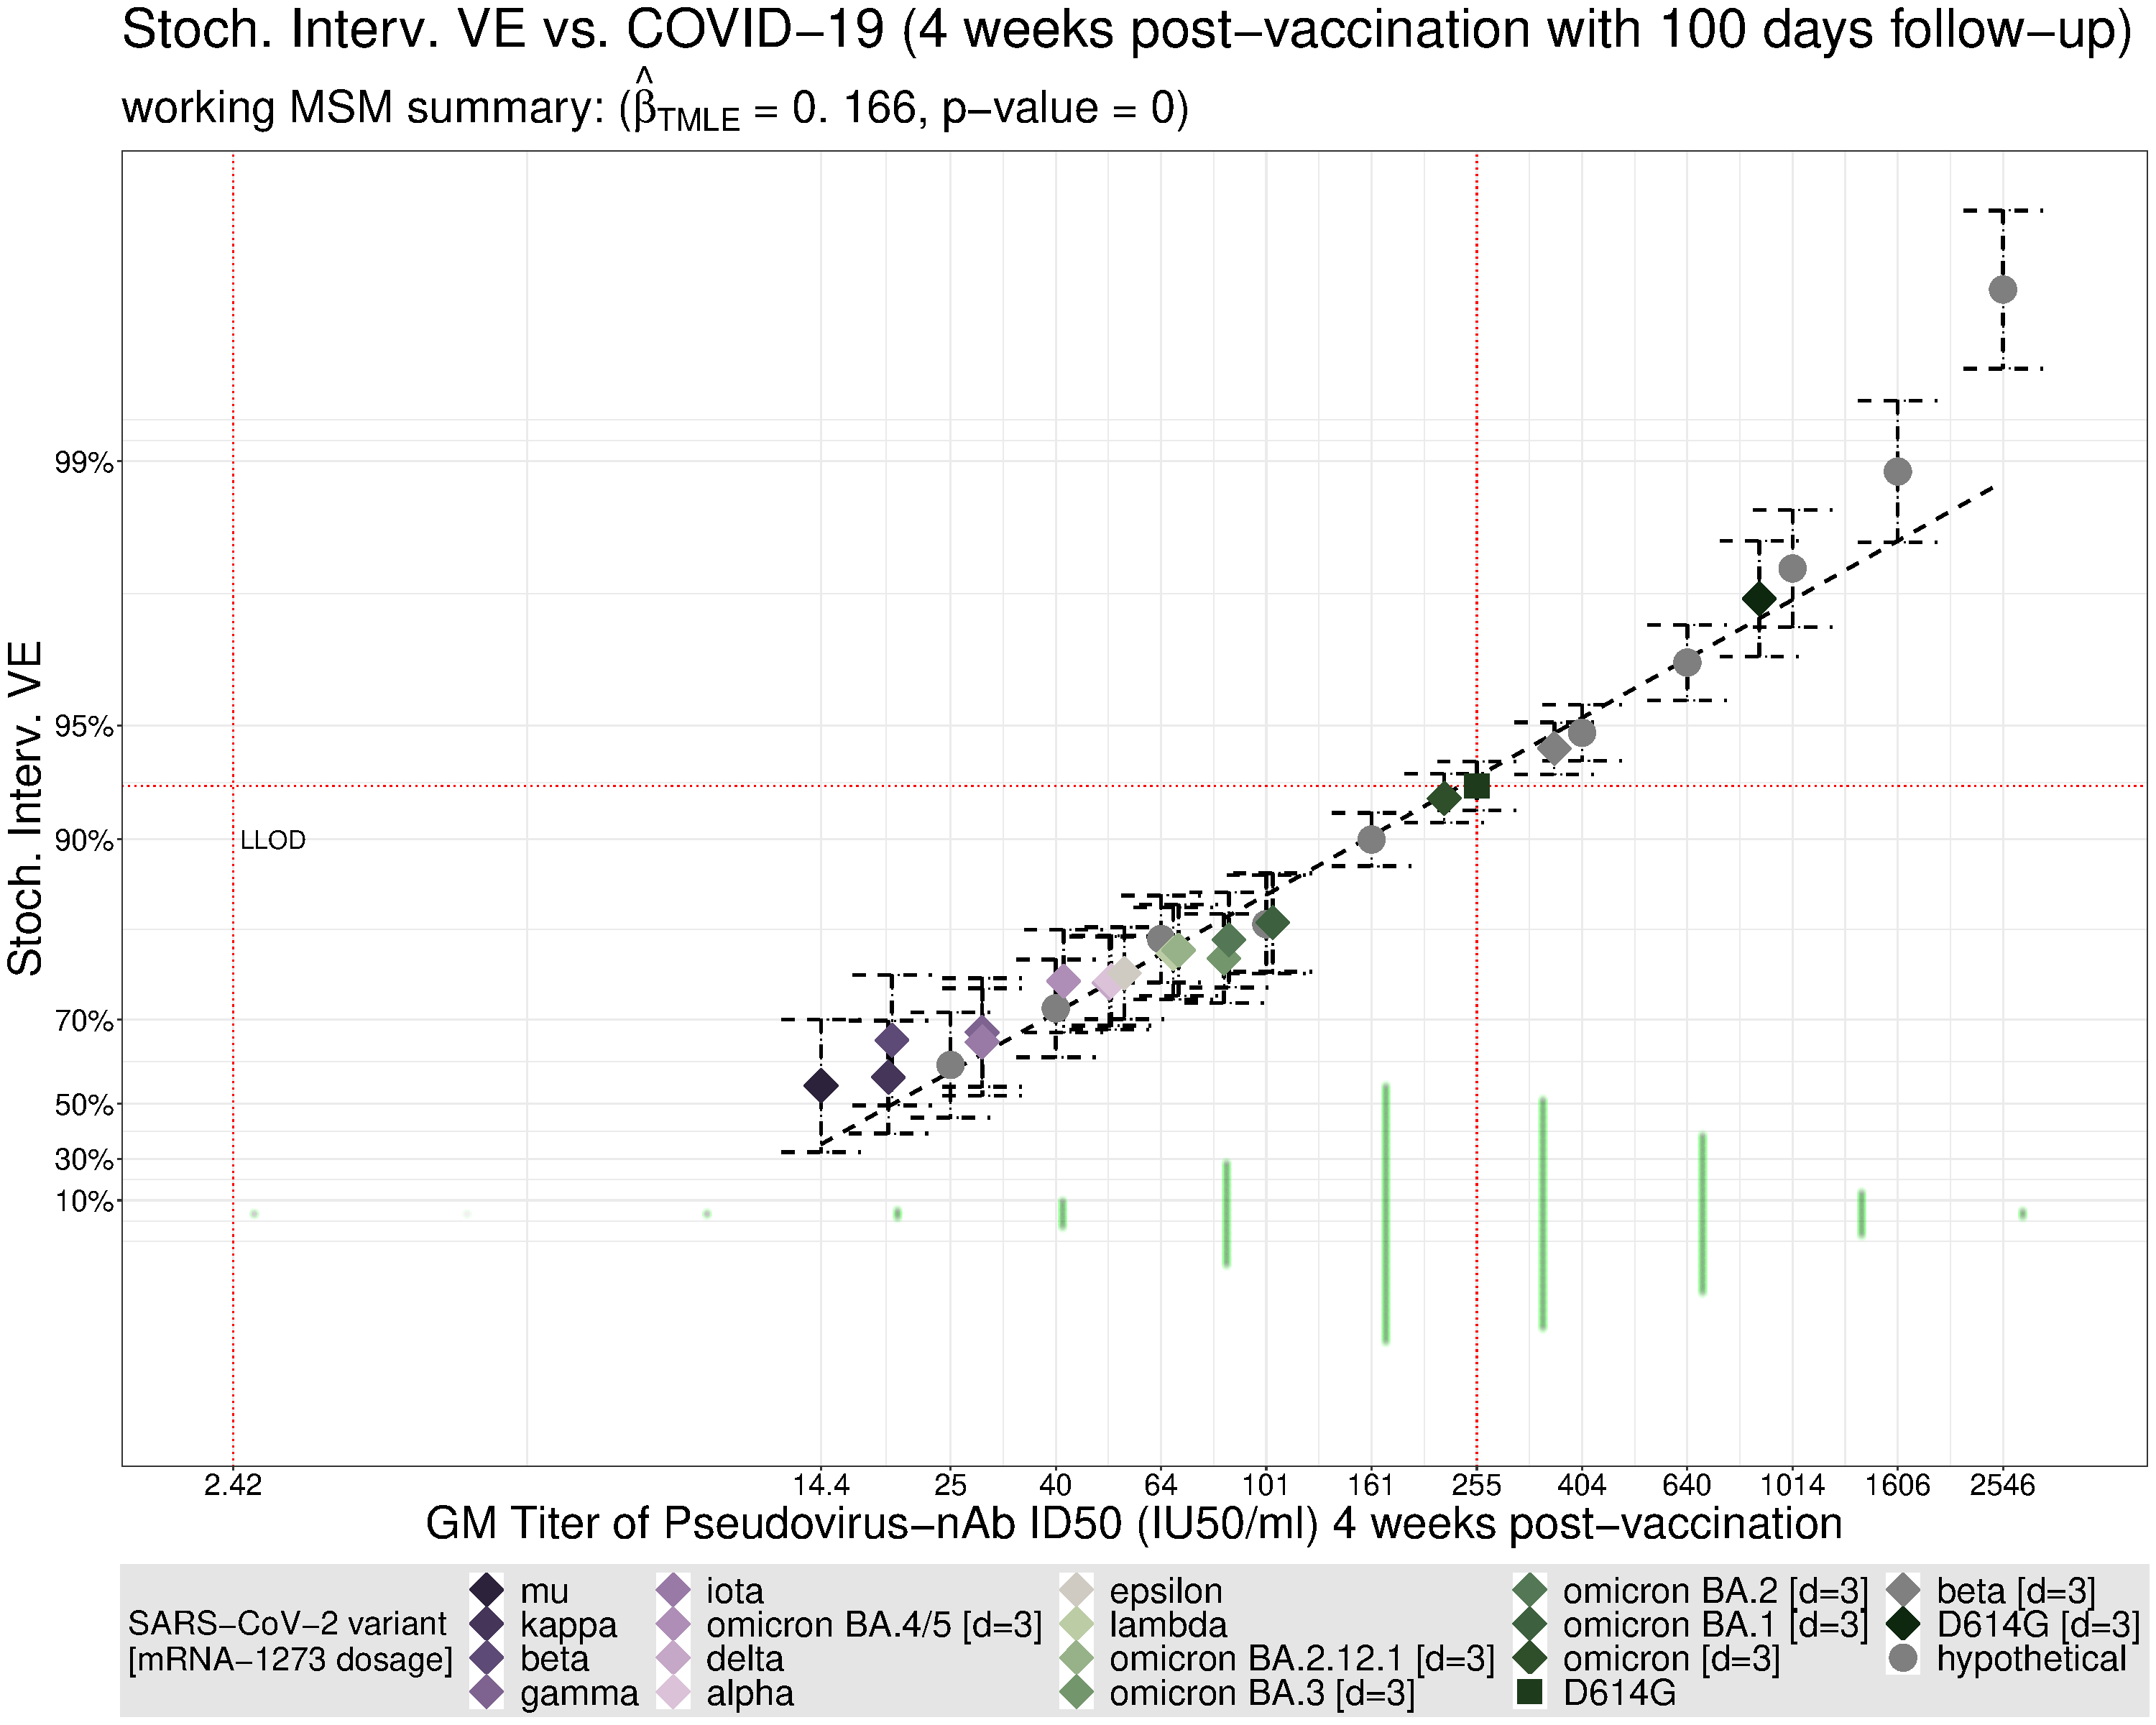
\includegraphics[scale=0.21]{sve_pseudoneutid50_immunobridging}

\note{
SVE is being measured for COVID-19 from 7-100 days post-4 weeks following
vaccination (Day 57 for 2 doses, Day 29 for 3 doses). Note that it is studying
the exact same data and time period as was studied in the \textit{Science}
paper.
}

\end{frame}

%%%%%%%%%%%%%%%%%%%%%%%%%%%%%%%%%%%%%%%%%%%%%%%%%%%%%%%%%%%%%%%%%%%%%%%%%%%%%%%%%

%\begin{frame}[c]{SVE Predictions vs.~Test-Negative Designs (TND) Estimates}

%\begin{center}
%\begin{itemize}
  %\itemsep6pt
  %\item Compared $\delta$-calibrated SVE predictions to TND VE estimates.
  %\item Inclusion/exclusion criteria for TND-based VE estimates\footnotemark:
    %\begin{itemize}
      %\itemsep2pt
      %\item VE estimated by direct measurement of SARS-CoV-2 variants.
      %\item Reported VE estimates for mRNA vaccines (BNT162b2 or mRNA-1273),
        %studying VE 2--6 months post-2\textsuperscript{nd} or
        %3\textsuperscript{rd} dose.
      %\item Flexible in choice of dosing interval (for 2\textsuperscript{nd} or
        %3\textsuperscript{rd} dose), with some studies extending to 12 weeks
        %between doses.
    %\end{itemize}
  %\item Aimed to study concordance of SVE predictions and TND estimates of VE
    %following most recent vaccine dose.
  %\item TND-based estimates established as biased (overestimating).
%\end{itemize}
%\end{center}

%\footnotetext[5]{\scriptsize Comparison of TND studies performed in
%collaboration with Dr.~Lindsay Carpp.}

%\note{
%}

%\end{frame}

%%%%%%%%%%%%%%%%%%%%%%%%%%%%%%%%%%%%%%%%%%%%%%%%%%%%%%%%%%%%%%%%%%%%%%%%%%%%%%%%

%\begin{frame}[c]{Comparison of SVE Predictions and TND Estimates of VE}

%\hspace*{-0.5cm}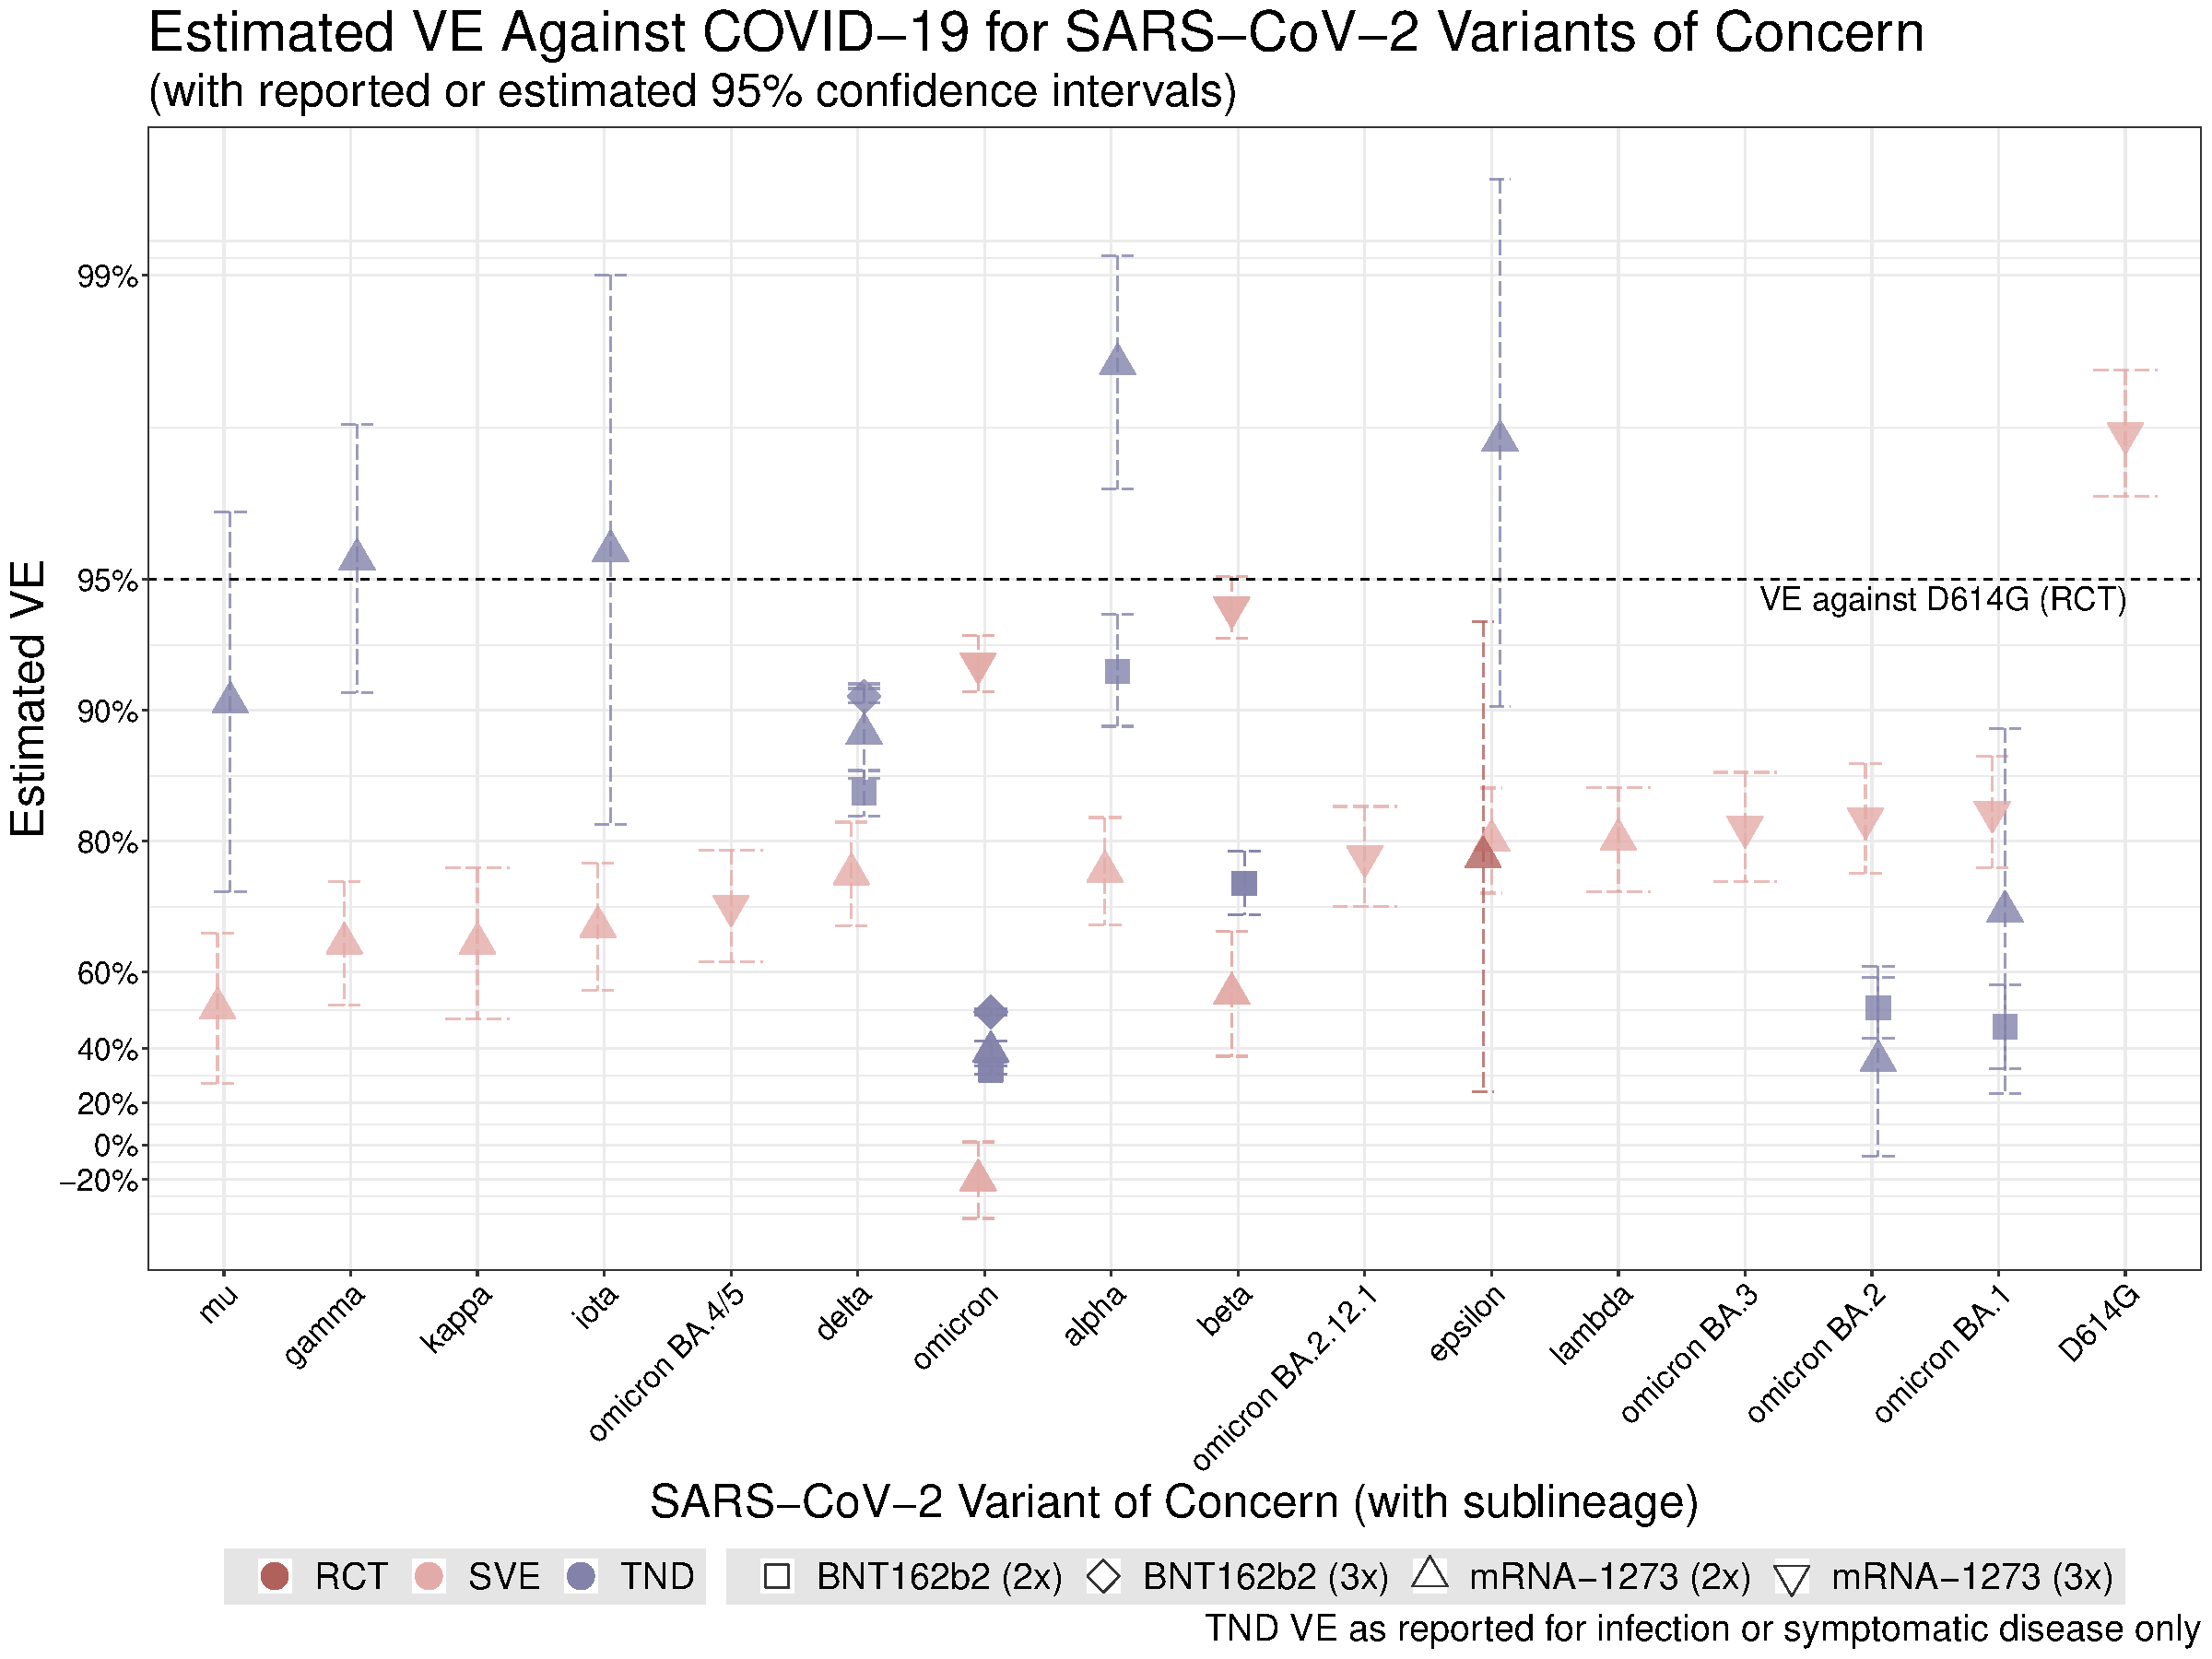
\includegraphics[scale=0.285]{tnd_sve_calib}

%\note{
%}

%\end{frame}

%%%%%%%%%%%%%%%%%%%%%%%%%%%%%%%%%%%%%%%%%%%%%%%%%%%%%%%%%%%%%%%%%%%%%%%%%%%%%%%%

%\begin{frame}[c]{Concordance of SVE Predictions and TND Estimates of VE}

%\hspace*{-0.5cm}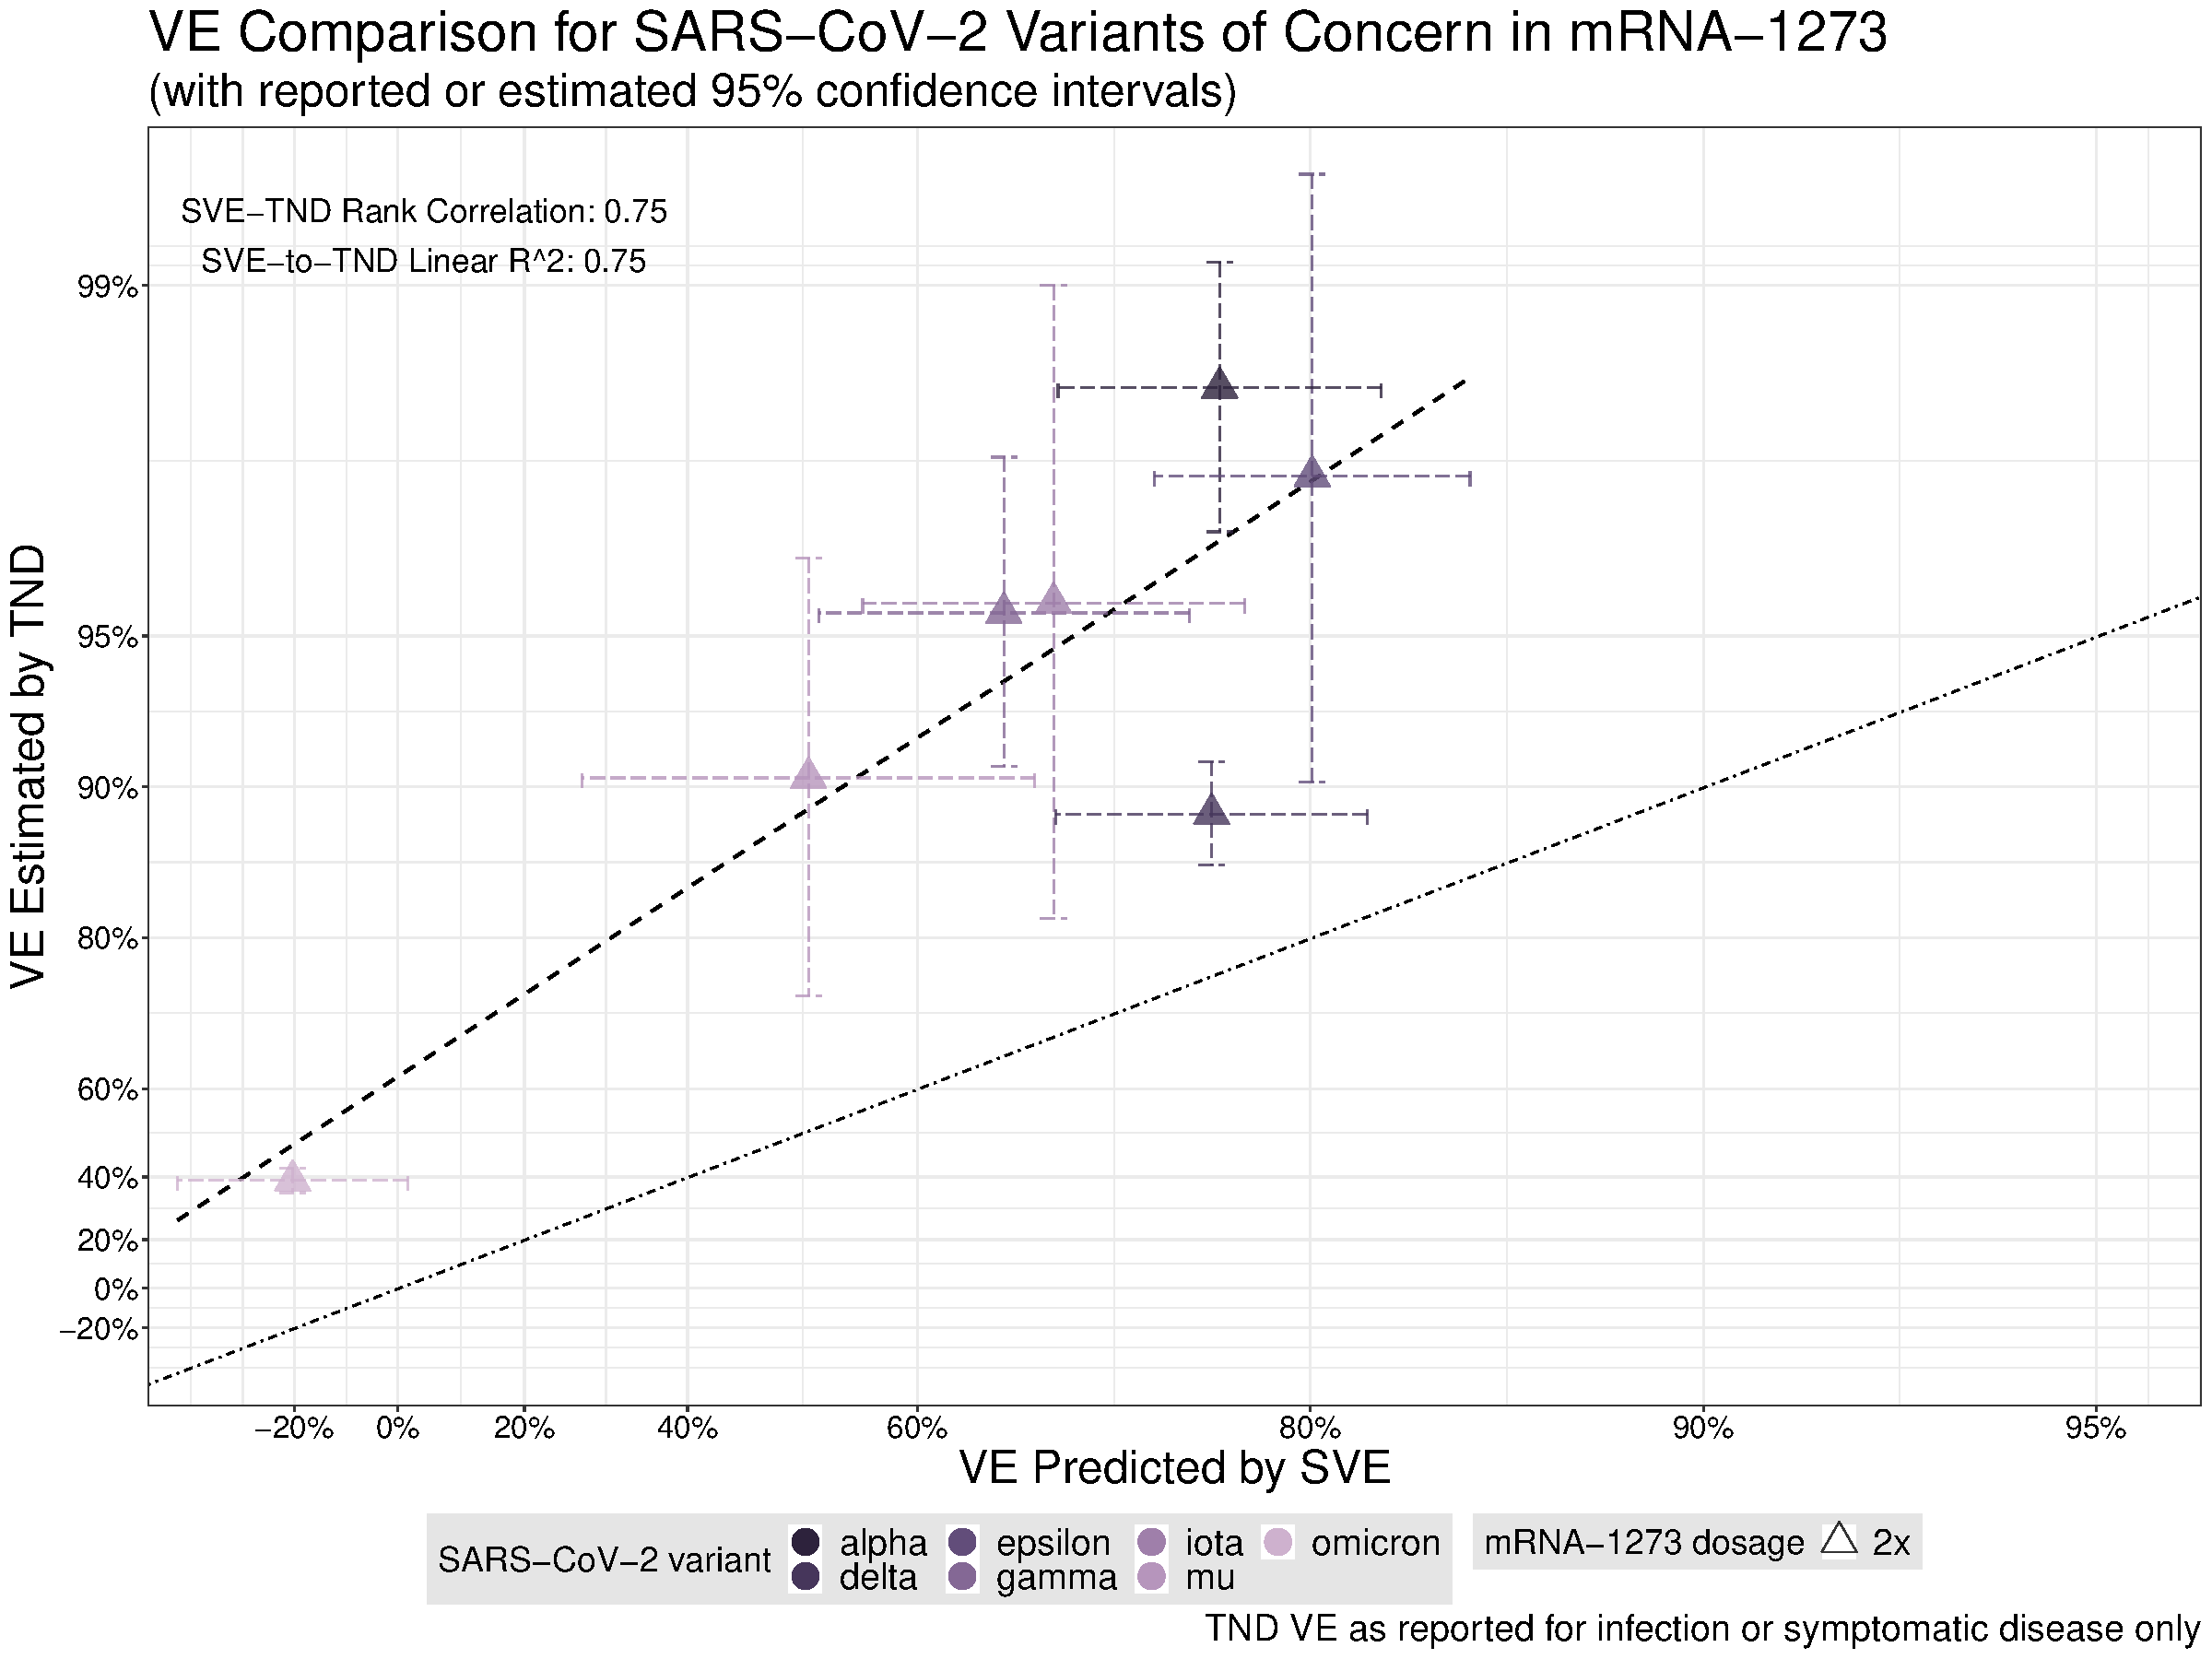
\includegraphics[scale=0.285]{tnd_sve_scatter}

%\note{
%}

%\end{frame}

%%%%%%%%%%%%%%%%%%%%%%%%%%%%%%%%%%%%%%%%%%%%%%%%%%%%%%%%%%%%%%%%%%%%%%%%%%%%%%%%

%\begin{frame}[c]{Summary of SVE for Prediction and Immunobridging}

%\begin{center}
%\begin{itemize}
  %\itemsep6pt
  %\item SVE prediction shows sharp changes in VE with shifts to the GM titer of
    %the PsV nAb correlate in vaccinees.
    %%\begin{itemize}
      %%\itemsep2pt
      %%\item Positive $\delta$: saturates at $\approx$100\%.
      %%\item Negative $\delta$: large range, from -20\%--92\%.
    %%\end{itemize}
  %\item Bridging VE across variants indicates VE drops but stabilizes at 50\%,
    %if the model based on ancestral D614G strain holds.
    %\begin{itemize}
      %\itemsep2pt
      %\item Post-2\textsuperscript{nd} dose: For most variants (excepting
        %omicron), the VE estimate ranges from 50\% (mu) to 80\% (epsilon).
      %\item Post-3\textsuperscript{rd} dose: For omicron lineages, VE estimate
        %lies within 80\%--92\% across five subvariants (lowest VE
        %vs.~BA.2.12.1).
    %\end{itemize}
  %%\item SVE predictions and TND estimates of VE well-correlated.
    %%\begin{itemize}
      %%\itemsep2pt
      %%\item TND studies are prone to bias, tending to overestimate VE.
      %%\item SVE predictions may be underestimates, since the PsV nAb correlate
        %%is an \textit{imperfect} causal \textit{mediator} of the total VE.
    %%\end{itemize}
%\end{itemize}
%\end{center}

%\note{
%}

%\end{frame}

%%%%%%%%%%%%%%%%%%%%%%%%%%%%%%%%%%%%%%%%%%%%%%%%%%%%%%%%%%%%%%%%%%%%%%%%%%%%%%%%

%\begin{frame}[standout]
  %Zooming Out
%\end{frame}

%%%%%%%%%%%%%%%%%%%%%%%%%%%%%%%%%%%%%%%%%%%%%%%%%%%%%%%%%%%%%%%%%%%%%%%%%%%%%%%

%\begin{frame}[c]{Going ``Off-Road'': Real-World Complexities}

%\begin{center}
%\begin{itemize}
  %\itemsep8pt
  %\item We considered the case of $O = (L, A, BS, Y, B)$, but what about $O =
    %(V, L, A, BS, Y, B)$ or $O = (L, A, Z, BS, Y, B)$?
    %\begin{itemize}
      %\item $Z$: \textit{unmeasured} baseline confounder (e.g., prior
        %infection)
      %\item $A \in \{0, 1\}$: randomized treatment assignment
      %\item $Z$: post-treatment confounder (e.g., unblinded risky
        %behavior)
      %\item $S$: candidate immune correlates (causal mediators)
      %\item $Y$: symptomatic SARS-CoV-2 (or HIV-1) infection
      %\item $B \coloneqq f(Y, L)$: selection into two-phase sample
    %\end{itemize}
  %\item And what about survival endpoints, $O = (L, A, BS, \Delta,
    %\widetilde{T}, B)$?
    %\begin{itemize}
      %\item $\widetilde{T} = \min(T_F, T_C)$: possibly right-censored time
        %to failure
      %\item $\Delta = \mathbb{I}(T_F < T_C)$: indicator of failure
        %endpoint occurrence
      %\item Could making $B$ a function of $\widetilde{T}$ improve sampling
        %efficiency?
    %\end{itemize}
%\end{itemize}
%\end{center}

%\note{
  %\begin{itemize}
  %\item Goal: assess \textit{indirect} effect of vaccination through mCoPs.
  %\item Define/identify new mCoPs to be used as surrogate endpoints.
  %\item Could also have missing outcome in the binary endpoint case.
  %\end{itemize}
%}

%\end{frame}

%%%%%%%%%%%%%%%%%%%%%%%%%%%%%%%%%%%%%%%%%%%%%%%%%%%%%%%%%%%%%%%%%%%%%%%%%%%%%%%%%

%\begin{frame}[c]{Towards Reproducible Statistical Data Science}
%\vspace{-0.5em}
%\textit{$\ldots$or ``What's wrong with that code I wrote that one time?''}

%\begin{center}
%\begin{itemize}
  %\itemsep6pt
  %%\item Open source packages and workflows for reproducible research in
    %%biomedical studies, with literate programming/computing.
  %\item Open source development: ongoing, continuous, public peer review of
    %research products --- a key to transparent science.
  %\item Scientific computing is \underline{not} an ancillary activity: the
    %bridge between statistical methods and their scientific application.
  %\item Recent and relevant contributions and collaborations:
    %\begin{itemize}
      %\itemsep2pt
      %\item \url{https://github.com/nhejazi/haldensify} -- \texttt{R} package
        %for conditional density estimation ($g_{0,S}$), novel estimators of
        %$\psi_{0,\delta}$.
      %\item \url{https://github.com/nhejazi/txshift} -- \texttt{R} package for
        %one-step, TML estimators of $\psi_{0,\delta}$, plus two-phase sampling.
      %%\item Co-design of statistical analysis suite for immune correlates
        %%analyses --- focusing on modularity and reproducibility.
    %\end{itemize}
%\end{itemize}
%\end{center}

%\note{
%}

%\end{frame}

%%%%%%%%%%%%%%%%%%%%%%%%%%%%%%%%%%%%%%%%%%%%%%%%%%%%%%%%%%%%%%%%%%%%%%%%%%%%%%%%%

%\begin{frame}[c]{Zooming Out: The Bigger Picture}

%\begin{center}
%\begin{itemize}
  %\itemsep8pt
  %\item Stochastic interventions provide a framework for formulating novel
    %policies based on natural treatment conditions.
  %\item These modified treatment policies address causal questions about
    %\textit{realistic} interventions on quantitative treatments.
  %\item Large-scale vaccine trials rely upon two-phase designs --- but need to
    %(very carefully!) adjust for the resultant sampling bias.
  %\item Efficient estimators with double/multiple robustness can safely answer
    %such questions \textit{while} incorporating machine learning.
  %\item Open source software for such statistical analyses is critical for the
    %methods to have any impact on real-world studies.
%\end{itemize}
%\end{center}

%\note{
%}

%\end{frame}

%%%%%%%%%%%%%%%%%%%%%%%%%%%%%%%%%%%%%%%%%%%%%%%%%%%%%%%%%%%%%%%%%%%%%%%%%%%%%%%%

%\begin{frame}[c]{Thank you}

%\Large{Thanks for listening. Any questions?}

%\vspace{2mm}
%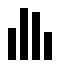
\includegraphics[scale=0.14]{homepage.png} \url{https://nimahejazi.org}

%\vspace{2mm}
%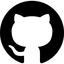
\includegraphics[scale=0.11]{github-icon.png}
  %\url{https://github.com/nhejazi}

%\vspace{2mm}
%
\includegraphics[scale=0.14]{twitter-icon.png}
  %\url{https://twitter.com/nshejazi}

%\end{frame}

%%%%%%%%%%%%%%%%%%%%%%%%%%%%%%%%%%%%%%%%%%%%%%%%%%%%%%%%%%%%%%%%%%%%%%%%%%%%%%%

%\appendix
%\begin{frame}[standout]
  %Appendix
%\end{frame}

%%%%%%%%%%%%%%%%%%%%%%%%%%%%%%%%%%%%%%%%%%%%%%%%%%%%%%%%%%%%%%%%%%%%%%%%%%%%%%%%

%\begin{frame}[c]{Immune Correlates of
  %Protection~\citep{plotkin2012nomenclature}}

%\begin{center}
%\begin{itemize}
  %\itemsep8pt
  %\item Correlate of Protection (CoP): immune marker statistically predictive
    %of vaccine efficacy, not necessarily mechanistic.
  %\item Mechanistic CoP (mCoP): immune marker that is causally and
    %mechanistically responsible for protection.
  %\item Nonmechanistic CoP (nCoP): immune marker that is predictive but not a
    %causal agent of protection.
  %\item A CoP is a \textit{candidate surrogate}
      %endpoint~\citep{prentice1989surrogate} --- primary
      %endpoint in future trials if reliably predictive.
%\end{itemize}
%\end{center}

%\note{
%}

%\end{frame}

%%%%%%%%%%%%%%%%%%%%%%%%%%%%%%%%%%%%%%%%%%%%%%%%%%%%%%%%%%%%%%%%%%%%%%%%%%%%%%%%

%\begin{frame}[c]{From the Causal to the Statistical Target Parameter}

%\begin{center}
%\begin{tcolorbox}
%\begin{assumption}{1}{\textit{Stable Unit Treatment Value (SUTVA)}}\label{sutva}
  %\begin{itemize}
    %\itemsep2pt
    %\item $Y^{d(s_i, l_i)}_i$ does not depend on $d(s_j, l_j)$ for
        %$i = 1, \ldots, n$ and $j \neq i$, or lack of
        %interference~\citep{cox1958planning}
        %%\citep{rubin1978bayesian, rubin1980randomization}
     %\item $Y^{d(s, l)} = Y$ in the event $S = d(s, l)$, for $i = 1, \ldots, n$
  %\end{itemize}
%\end{assumption}
%\end{tcolorbox}
%\vspace{-0.7em}
%\begin{tcolorbox}
%\begin{assumption}{2}{\textit{No Unmeasured Confounding}}\label{ignorability}
  %$S \indep Y^{d(s, l)} \mid L = l$, for $i = 1, \ldots, n$
%\end{assumption}
%\end{tcolorbox}
%\vspace{-0.7em}
%\begin{tcolorbox}
%\begin{assumption}{3}{\textit{Positivity}}\label{positivity}
  %$s \in \mathcal{S} \implies d(s, l) \in \mathcal{S}$ for all
  %$l \in \mathcal{L}$, where $\mathcal{S}$ denotes the support of $S$
  %conditional on $L = l$ for all $i = 1, \ldots n$
%\end{assumption}
%\end{tcolorbox}
%\end{center}

%\note{
%\begin{itemize}
  %\itemsep4pt
  %\item This positivity assumption is not quite the same as that required for
    %categorical interventions.
  %\item In particular, we do not require that the intervention density place
    %mass across all strata defined by $L$.
  %\item Rather, we merely require the post-intervention quantity be seen in the
    %observed data for given $s_i \in \mathcal{S}$ and $l_i \in \mathcal{L}$.
%\end{itemize}
%}

%\end{frame}

%%%%%%%%%%%%%%%%%%%%%%%%%%%%%%%%%%%%%%%%%%%%%%%%%%%%%%%%%%%%%%%%%%%%%%%%%%%%%%%%

%\begin{frame}[c]{Literature: \cite{diaz2012population, diaz2018stochastic}}

%\begin{center}
%\begin{itemize}
  %\itemsep8pt
  %\item \textit{Proposal:} Evaluate outcome under an altered
    %\textit{intervention distribution} --- e.g.,
    %$P_{\delta}(g_{0,S})(S = s \mid L) = g_{0,S}(s - \delta(L) \mid L)$.
  %\item Identification conditions for a statistical parameter of the
    %counterfactual outcome $\psi_{0,\delta}$ under such an intervention.
  %\item Show that the causal quantity of interest $\E_{P_0^{\delta}}
    %\{Y_{d(S, L)}\}$ is identified by a functional of the distribution of $O$,
    %i.e.,
    %\begin{align*}\label{eqn:identification2012}
      %\psi_{0,\delta} = \int_{\mathcal{L}} \int_{\mathcal{S}} &\E_{P_0}
        %\{Y \mid S = d(s, l), L = l\} \\ &g_{0, S}(s \mid L = l) \cdot
        %q_{0, L}(l) d\mu(s)d\nu(l)
    %\end{align*}
%\end{itemize}
%\end{center}

%\note{
  %\begin{itemize}
    %\item The identification result allows us to write down the causal quantity
      %of interest in terms of a functional of the observed data.
    %\item Key innovation: loosening standard assumptions through a change in
      %the observed intervention mechanism.
    %\item Problem: globally altering an intervention mechanism does not
      %necessarily respect individual characteristics.
    %\item The authors build IPW, one-step, and TML estimators, comparing the
      %three different approaches.
  %\end{itemize}
%}

%\end{frame}

%%%%%%%%%%%%%%%%%%%%%%%%%%%%%%%%%%%%%%%%%%%%%%%%%%%%%%%%%%%%%%%%%%%%%%%%%%%%%%%%

%\begin{frame}[c]{Literature: \cite{haneuse2013estimation}}

%\begin{center}
%\begin{itemize}
  %\itemsep8pt
  %\item \textit{Proposal:} Characterization of stochastic interventions as
    %\textit{modified treatment policies} (MTPs).
  %\item Assumption of \textit{piecewise smooth invertibility} allows for the
    %post-intervention distribution of any MTP to be recovered:
    %\begin{equation*}
      %g_{0, S}(s \mid l; \delta) = \sum_{j = 1}^{J(l)} \mathbb{I}_{\delta, j}
      %\{h_j(s, l), l\} g_0\{h_j(s, l) \mid l\} h^{'}_j(s, l)
    %\end{equation*}
  %\item MTPs account for the natural value of exposure $S$ yet may be
    %interpreted as imposing an altered intervention mechanism.
%\end{itemize}
%\end{center}

%\note{
  %\begin{itemize}
    %\item Shifts of the form $\delta(S, L)$ are considerably more interesting
      %since these are realistic intervention policies.
    %\item Example: consider an individual with an extremely high immune response
      %but whose baseline covariates $L$ suggest we shift the response still
      %higher. Such a shift may not be biologically plausible (impossible, even)
      %but we cannot account for this if the shift is only a function of $L$.
    %\item The authors build IPW, outcome regression, and non-iterative doubly
      %robust estimators, as well as an approach based on MSMs.
    %\item Piecewise smooth invertibility: This assumption ensures that we can
      %use the change of variable formula when computing integrals over $S$ and
      %it is useful to study the estimators that we propose in this paper.
  %\end{itemize}
%}

%\end{frame}

%%%%%%%%%%%%%%%%%%%%%%%%%%%%%%%%%%%%%%%%%%%%%%%%%%%%%%%%%%%%%%%%%%%%%%%%%%%%%%%%

%\begin{frame}[c]{Literature: \cite{young2014identification}}

%\begin{center}
%\begin{itemize}
  %\itemsep8pt
  %\item Establishes equivalence between g-formula when proposed intervention
    %depends on natural value and when it does not.
  %\item This equivalence leads to a sufficient positivity condition for
    %estimating the counterfactual mean under MTPs via the same statistical
    %functional studied in \cite{diaz2012population}.
  %\item Extends earlier identification results, providing a way to use the same
    %statistical functional to assess $\E Y_{d(S,L)}$ or $\E Y_{d(L)}$.
  %\item The authors also consider limits on implementing shifts $d(S,L)$, and
    %address working in a longitudinal setting.
%\end{itemize}
%\end{center}

%\note{
%}

%\end{frame}

%%%%%%%%%%%%%%%%%%%%%%%%%%%%%%%%%%%%%%%%%%%%%%%%%%%%%%%%%%%%%%%%%%%%%%%%%%%%%%%%

%\begin{frame}[c]{A Linear Modeling Perspective}

%\begin{center}
%\begin{itemize}
  %\itemsep6pt
  %\item Briefly consider a simple data structure: $X = (Y, S)$; we seek to model
    %the outcome $Y$ as a function of $S$.
  %\item Linear model: consider $Y_i = \beta_0 + \beta_1 S_i + \epsilon_i$, with
    %error $\epsilon_i \sim N(0, 1)$.
  %\item Letting $\delta$ be a change in $S$, $Y_{S + \delta} - Y_S$ may be
    %expressed
    %\begin{align*}
      %\E Y_{S + \delta} - \E Y_S &= [\beta_0 + \beta_1 (\E S + \delta)] -
        %[\beta_0 + \beta_1 (\E S)] \\
        %&= \beta_0 - \beta_0 + \beta_1 \E S - \beta_1 \E S + \beta_1 \delta \\
        %&= \beta_1 \delta
    %\end{align*}
  %\item So, a \textit{unit shift} in $S$ (i.e., $\delta = 1$) induces a
    %change in the difference in outcomes of magnitude $\beta_1$.
%\end{itemize}
%\end{center}

%\note{
  %\begin{itemize}
    %\item We extend this result to the mean counterfactual outcomes under the
      %nonparametric model $\M$.
  %\end{itemize}
%}

%\end{frame}

%%%%%%%%%%%%%%%%%%%%%%%%%%%%%%%%%%%%%%%%%%%%%%%%%%%%%%%%%%%%%%%%%%%%%%%%%%%%%%%%

%\begin{frame}[c]{Slope in a Semiparametric Model}

%\begin{center}
%\begin{itemize}
  %\itemsep8pt
  %\item Consider the stochastic intervention $g_{\delta}(\cdot \mid L)$:
    %\begin{align*}
      %\E Y_{g_{\delta}} &= \int_L \int_s \E(Y \mid S = s, L) g(s - \delta
            %\mid L) ds dP_0(L) \\
        %&= \int_L \int_z \E(Y \mid S = z + \delta, L) g(z \mid L) dz dP_0(L),
    %\end{align*}
      %defning the change of variable $z = s - \delta$.
  %\item For a semiparametric model, $\E (Y \mid S = z, L) = \beta z +
    %\theta(L)$:
    %\begin{align*}
      %\E Y_{g_{\delta}} - \E Y &= \int_L \int_z
      %\begin{aligned}[t]
        %& [\E(Y \mid S = z + \delta, L) - \E(Y \mid S = z, L)] \\
        %& g(z \mid L) dz dP_0(L)
      %\end{aligned} \\
      %&= [\beta (z + \delta) + \theta(L)] - [\beta z + \theta(L)] \\
      %&= \beta \delta
    %\end{align*}
%\end{itemize}
%\end{center}

%\note{
%}

%\end{frame}

%%%%%%%%%%%%%%%%%%%%%%%%%%%%%%%%%%%%%%%%%%%%%%%%%%%%%%%%%%%%%%%%%%%%%%%%%%%%%%%%

%\begin{frame}[c]{Flexible Conditional Density Estimation of $g_{0,S}$}

%\begin{center}
%\begin{itemize}
  %\itemsep8pt
  %\item \cite{diaz2011super}'s conditional density estimator:
    %\begin{equation*}
      %g_{n, \alpha}(s \mid L) = \frac{\pr (s \in [\alpha_{t-1}, \alpha_t)
        %\mid L)}{\alpha_t - \alpha_{t-1}}.
    %\end{equation*}
    %%for $\alpha_{t-1} \leq s < \alpha_t$.
    %\vspace{-0.5em}
    %\begin{itemize}
      %\itemsep4pt
      %\item Re-expressed as hazard regressions in repeated measures data.
      %\item Tuning parameter $t$ $\approx$ bandwidth in kernel density
        %estimation.
    %\end{itemize}
  %\item When c\`{a}dl\`{a}g (RCLL) with finite sectional variation, we have
    %{\small{
    %\begin{equation*}
     %\logit \{\pr(s \in [\alpha_{t-1}, \alpha_t) \mid L)\} = \beta_0 +
       %\sum_{w \subset\{1,\ldots,d\}} \sum_{i=1}^{n} \beta_{w,i} \phi_{w,i},
    %\end{equation*} }
    %}
    %for appropriate basis functions
    %$\{ \phi_{w,i} \}_{i=1}^n$~\citep{gill1995inefficient}.
%\end{itemize}
%\end{center}

%\note{
%}

%\end{frame}

%%%%%%%%%%%%%%%%%%%%%%%%%%%%%%%%%%%%%%%%%%%%%%%%%%%%%%%%%%%%%%%%%%%%%%%%%%%%%%%

%\begin{frame}[c]{Flexible Conditional Density Estimation of $g_{0,S}$}

%\begin{center}
%\begin{itemize}
  %\itemsep8pt
  %\item Utilizing a particular basis construction for $\phi_w$,
    %\citet{vdl2017generally}'s HAL estimator achieves $n^{-1/4}$
    %convergence rate\footnotemark.
  %\item Loss-based cross-validation allows selection of a suitable HAL
    %estimator, which has only the $\ell_1$ regularization term $\lambda$:
    %{\small{
    %\begin{equation*}
      %\beta_{n, \lambda}= \argmin_{\beta: \lvert \beta_0 \rvert + \sum_{w
        %\subset\{1,\ldots,d\}} \sum_{i=1}^{n} \lvert \beta_{w,i} \rvert <
        %\lambda} P_n \lik(g_{\beta,\lambda,S}),
    %\end{equation*} }
    %}
    %where $\lik(\cdot)$ is an appropriate loss function, giving
    %$\{\lambda_n, \beta_n\}$.
  %\item We denote by $g_{n,\lambda,S} \coloneqq g_{\beta_{n, \lambda},S}$, the
    %HAL estimate of $g_{0,S}$.
  %\item Our \texttt{haldensify} \texttt{R} package implements our estimator of
    %$g_{0,S}$.
%\end{itemize}
%\end{center}

%\note{
%\begin{itemize}
  %\item C\`{a}dl\`{a}g: right-hand continuous with left-hand limits
  %\item Improved convergence rate~\citep{bibaut2019fast}:
    %\begin{equation*}
      %\lvert \theta_{n,M_n} - \theta_{0} \rvert_{P_0} =
      %o_P(n^{-1/3} \log(n)^{d/2}) \ .
    %\end{equation*}
%\end{itemize}
%}

%\footnotetext[6]{Similar rates can be achieved via \textit{local} (vs.~global)
%smoothness assumptions on $g_{n,S}$~\citep[see, e.g.,][]{robins2008higher,
%mukherjee2017semiparametric, liu2021adaptive}.
%}

%\end{frame}

%%%%%%%%%%%%%%%%%%%%%%%%%%%%%%%%%%%%%%%%%%%%%%%%%%%%%%%%%%%%%%%%%%%%%%%%%%%%%%%

%\begin{frame}{A Useful Class of Functions}
%\vspace{0.75cm}

%Consider space of \textit{cadlag} functions with \textit{finite variation
%norm}.

%\textbf{Def.} cadlag = \textit{left-hand continuous} with
%\textit{right-hand limits}
%\vspace{0.25cm}

%\textbf{Variation norm}
%Let $\theta_s(u)=\theta(u_s,0_{s^c})$ be the \textit{section} of $\theta$ that
%sets the coordinates in $s$ \textit{equal to zero}.
%\vspace{0.15cm}

%The \textit{variation norm} of $\theta$ can be written:
%\[
  %\lvert \theta \rvert_v=\sum_{s\subset\{1,\dots,d\}}\int \mid
  %d\theta_s(u_s)\mid ,
%\]
%where $x_s=(x(j):j\in s)$ and the sum is over all subsets.

%\note{
%}

%\end{frame}

%%%%%%%%%%%%%%%%%%%%%%%%%%%%%%%%%%%%%%%%%%%%%%%%%%%%%%%%%%%%%%%%%%%%%%%%%%%%%%%

%\begin{frame}{Variation Norm}

%We can represent the function $\theta$ as
%\begin{eqnarray*}
%\theta(x)&=&\theta(0) + \sum_{s\subset\{1,\ldots,d\}}
  %\int \I(x_s\geq u_s)d\theta_s(u_s),
%\end{eqnarray*}

%For discrete measures $d\theta_s$ with \textit{support points} $\{u_{s,j}:j\}$
%we get a \textit{linear combination} of indicator \textit{basis functions}:
%\[
  %\theta(x) = \theta(0) + \sum_{s\subset\{1,\ldots,d\}}\sum_{j} \beta_{s,j}
    %\theta_{u_{s,j}}(x),
%\]
%where $\beta_{s,j}=d\theta_s(u_{s,j})$,
%$\theta_{u_{s,j}}(x) = \I(x_s \ge u_{s,j})$,
%and
%\begin{equation*}
%\lvert \theta \rvert_v = \theta(0) + \sum_{s\subset\{1,\ldots,d\}}
  %\sum_j \lvert \beta_{s,j} \rvert.
%\end{equation*}

%\note{
%}

%\end{frame}

%%%%%%%%%%%%%%%%%%%%%%%%%%%%%%%%%%%%%%%%%%%%%%%%%%%%%%%%%%%%%%%%%%%%%%%%%%%%%%%

%\begin{frame}{Convergence Rate of HAL}
%\vspace{0.25cm}

%We have, for $\alpha(d)=1/(d+1)$,
%\[
  %\lvert \theta_{n,M} - \theta_{0,M} \rvert_{P_0}=o_P(n^{-(1/4+\alpha(d)/8)}).
%\]

%Thus, if we select $M> \lvert \theta_0 \rvert_v$, then
%\[
  %\lvert \theta_{n,M} - \theta_{0} \rvert_{P_0} =
  %o_P(n^{-(1/4+\alpha(d)/8)})\ .
%\]

%Due to oracle inequality for the cross-validation selector $M_n$,
%\[
  %\lvert \theta_{n,M_n} - \theta_{0} \rvert_{P_0} =
  %o_P(n^{-(1/4+\alpha(d)/8)}) \ .
%\]

%Improved convergence rate~\citep{bibaut2019fast}:
%\[
  %\lvert \theta_{n,M_n} - \theta_{0} \rvert_{P_0} =
  %o_P(n^{-1/3} \log(n)^{d/2}) \ .
%\]

%\note{
  %\begin{itemize}
  %\item The goal was to construct nuisance parameter estimators that are
    %\textit{consistent} and \textit{converge faster} than $n^{-1/4}$ under
    %\textit{minimal assumptions}.
  %\item We have assumed enough \textit{smoothness} that HAL will
    %\textit{converge faster} than $n^{-1/4}$, but retain enough flexibility
    %that \textit{consistency} is also preserved.
  %\end{itemize}
%}

%\end{frame}

%%%%%%%%%%%%%%%%%%%%%%%%%%%%%%%%%%%%%%%%%%%%%%%%%%%%%%%%%%%%%%%%%%%%%%%%%%%%%%%%

%\begin{frame}[c]{Algorithm for TML Estimation}

%\begin{center}
%\begin{enumerate}\label{tmle_algo}
  %\itemsep6pt
  %\item Construct initial estimators $g_n$ of $g_0(S, L)$ and $Q_n$ of
    %$\overline{Q}_0(S, L)$, perhaps using data-adaptive regression techniques.
  %\item For each observation $i$, compute an estimate $H_n(s_i, l_i)$ of the
    %auxiliary covariate $H(s_i, l_i)$.
  %\item Estimate the parameter $\epsilon$ in the logistic regression model
    %$$\text{logit}\overline{Q}_{\epsilon, n}(s, l) =
    %\text{logit}\overline{Q}_n(s, l) + \epsilon H_n(s, l),$$
    %or an alternative regression model incorporating weights.
  %\item Compute TML estimator $\Psi_n$ of the target parameter, defining update
    %$\overline{Q}_n^{\star}$ of the initial estimate
    %$\overline{Q}_{n, \epsilon_n}$:
    %\begin{equation*}\label{tmle}
      %\Psi_n = \Psi(P_n^{\star}) = \frac{1}{n} \sum_{i = 1}^n
        %\overline{Q}_n^{\star}(d(S_i, L_i), L_i).
      %\end{equation*}
%\end{enumerate}
%\end{center}

%\note{
  %\begin{itemize}
    %\item We recommend using nonparametric methods for the initial estimators,
      %as consistent estimation is necessary for efficiency of the estimator
      %$\Psi_n$.
    %\item Intuition for the submodel fluctuation?
  %\end{itemize}
%}

%\end{frame}

%%%%%%%%%%%%%%%%%%%%%%%%%%%%%%%%%%%%%%%%%%%%%%%%%%%%%%%%%%%%%%%%%%%%%%%%%%%%%%%%

%\begin{frame}[c]{Algorithm for IPCW-TML Estimation}

%\begin{center}
%\begin{enumerate}\label{ipcwtmle_algo}
  %\itemsep8pt
  %\item Using all observed units ($X$), estimate sampling mechanism
    %$\pi(Y, L)$, perhaps using data-adaptive regression methods.
  %\item Using only observed units in the second-stage sample $C = 1$,
    %construct initial estimators $g_n(S,L)$ and $\overline{Q}_n(S,L)$,
    %weighting by the sampling mechanism estimate $\pi_n(Y,L)$.
  %\item With the approach described for the full data case, compute
    %$H_n(s_i,l_i)$, and fluctuate submodel via logistic regression.
  %\item Compute IPCW-TML estimator $\Psi_n$ of the target parameter, by solving
    %the IPCW-augmented EIF estimating equation.
  %\item Iteratively update estimated sampling weights $\pi_n(Y,L)$ and
    %IPCW-augmented EIF, updating TMLE in each iteration.
%\end{enumerate}
%\end{center}

%\note{
  %\begin{itemize}
    %\item We recommend using nonparametric methods for the initial estimators,
      %as consistent estimation is necessary for efficiency of the estimator
      %$\Psi_n$.
    %\item Intuition for the submodel fluctuation?
    %\item This process includes the use of HAL to fit the regression of the EIF
      %contributions on the sampling node $\{Y, L\}$.
  %\end{itemize}
%}

%\end{frame}

%%%%%%%%%%%%%%%%%%%%%%%%%%%%%%%%%%%%%%%%%%%%%%%%%%%%%%%%%%%%%%%%%%%%%%%%%%%%%%%%

% don't want dimming with references
\setbeamercovered{}
\beamerdefaultoverlayspecification{}

\begin{frame}[c,allowframebreaks]{}

\tiny
\bibliographystyle{apalike}
%\nocite{*}
\bibliography{references}
\itemize

\end{frame}

%%%%%%%%%%%%%%%%%%%%%%%%%%%%%%%%%%%%%%%%%%%%%%%%%%%%%%%%%%%%%%%%%%%%%%%%%%%%%%%%
\end{document}
